%\documentclass[pageno]{jpaper}
%
%%replace XXX with the submission number you are given from the ASPLOS submission site.
%\newcommand{\asplossubmissionnumber}{1141}
%\usepackage{caption}
%\usepackage{subcaption}
%\usepackage[normalem]{ulem}
%
%%\usepackage[firstpage]{draftwatermark}
%%\SetWatermarkText{ASPLOS'21 \#\asplossubmissionnumber: DO NOT DISTRIBUTE}
%%\SetWatermarkColor[gray]{0.8}
%%\SetWatermarkScale{0.25}
%
%\begin{document}
%
%\title{Exploiting Image Resolution for Inference System Optimizations}
%
%\date{}
%\maketitle
%
%\thispagestyle{empty}
%
%\begin{abstract}
%
%Image resolution has significant impact on accuracy and the computational, storage, and bandwidth costs of computer vision model inference.
%These costs are exacerbated when scaling out models to large inference serving systems and make image resolution an attractive target for inference systems optimizations.
%However, the choice of resolution inherently introduces additional tightly coupled choices, such as image crop size, image detail, and compute kernels that impact computational, storage, and bandwidth costs.
%%To understand these tradeoff space defined by these parameters, characterize image resolution as a basic hyperparameter of convolutional neural network inference and how we can leverage a resolution-aware stack to make favorable tradeoffs in both storage (capacity and access bandwidth) and computation.
%We characterize this tradeoff space by proposing a method and a set of mechanisms for multi-resolution support that takes advantage of how image codecs arrange image data and autotuning of convolutional neural network operators.
%We propose and evaluate support for efficient multi-resolution image inference in terms of model accuracy, storage (bytes of image data read), computation (wall-clock time and FLOPs), spanning image formats, compute kernel tuning, and model pipelines.
%Additionally, we evaluate a dynamic resolution approach that removes the need to statically choose a resolution ahead of time, finding a favorable accuracy vs. compute cost tradeoff.
%We show that autotuning kernels at low resolutions can improve throughput by up to 40\% at low resolution inference, up to 20-30\% of image data can be ignored (reducing storage bandwidth pressure) without losing model accuracy at high resolution inference (even given modestly sized input images), and decreasing the crop size can boost model accuracy by up to 5\% at low resolutions.
%\end{abstract}

\section{Introduction}
\begin{figure}
    \centering
    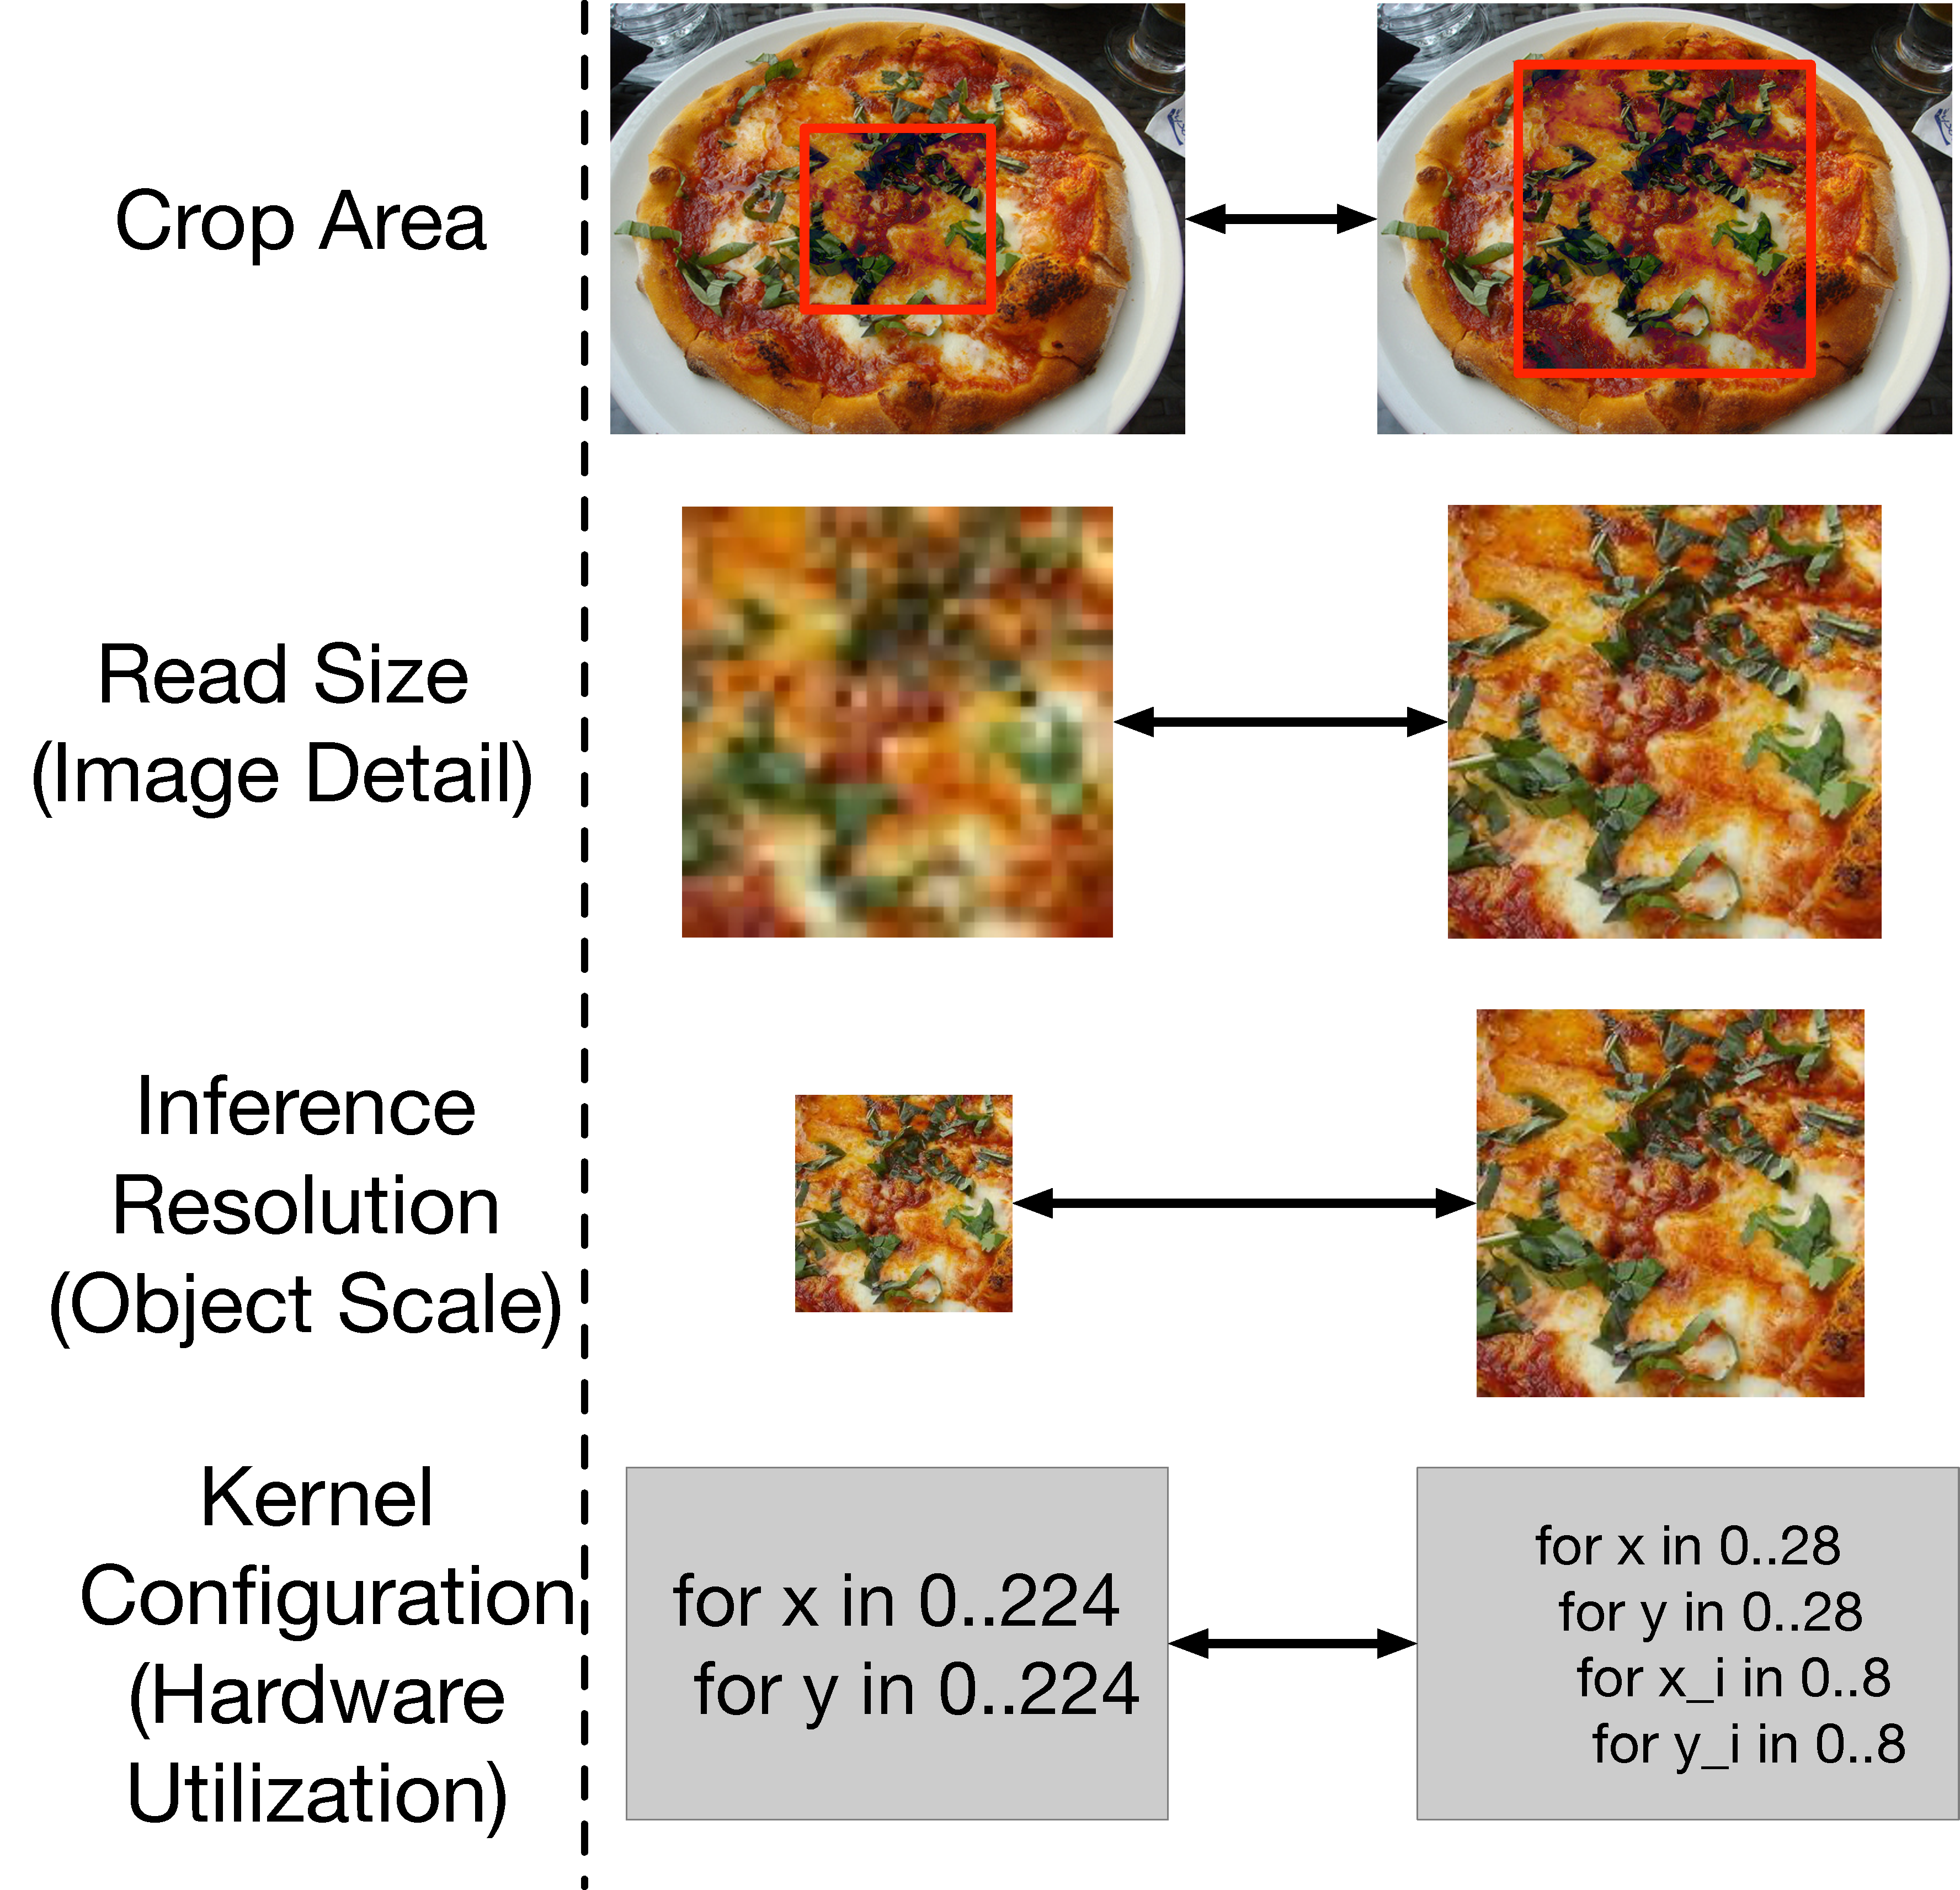
\includegraphics[width=\textwidth]{e2e_diagrams/tradeoff space.pdf}
    \caption{The choice of inference resolution in neural networks introduces associated tightly coupled choices, controlling properties such as the apparent size of objects (crop area), image detail (read size), and inference latency (compute kernel configuration). Each choice potentially impacts one or more of model accuracy, inference time, and data storage bandwidth.}
    \label{fig:tradeoffs}
\end{figure}

The choice of image resolution is an important hyperparameter for neural networks.
Input images for computer vision models typically comprise a wide range of resolutions, qualities, and object scales, yet the choice of input resolution is typically a static one.
Furthermore, computation and memory requirements scale approximately quadratically with input resolution, increasing the cost of scaling input resolution dramatically.
In this work, we claim that image resolution is an underexploited hyperparameter in neural network models, and quantify the impact that the choice of resolution has on system resources such as compute throughput and storage bandwidth.
We frame the choice of neural network resolution at inference time as existing in a space of many related parameters, such as crop area, the quantity of data to read, and the configuration of compute kernels (\autoref{fig:tradeoffs}).
We study questions about the impact of image resolution in the static resolution setting, followed by the question of whether image resolution can be a dynamic choice.
 
%improvements from full-stack dynamic image-resolution awareness in model inference pipelines.
%We begin by motivating the need for dynamic or multi-resolution inference pipelines  in terms of model accuracy.
%Next, we show techniques to minimize the bytes of image data read from storage and wall-clock time used for computation while improving model accuracy by leveraging image resolution dynamically at inference time.
%Along the way, we show that even in the absence of dynamism, our approach can be used to optimize static pipelines with respect to storage and computation.

\paragraph{What is The Impact of Image Resolution?}
Modern computer vision models typically run at a fixed resolution, with this resolution often chosen in tandem with the model architecture.
While recent work has drawn attention to the importance of proper resolution scaling with respect to computational cost and model accuracy~\cite{tan2019efficientnet}, the true wall-clock latency impact on inference systems remains ambiguous.
When scaling the input resolution of a model, the number of arithmetic operations incurred by increasing floating-point operations can be easily counted, but it is unclear whether hardware utilization is identical across all resolutions such that wall-clock time scales commensurately.
Additionally, storage capacity and bandwidth are precious resources that are intertwined with image resolution, raising additional questions regarding the quantity of image data that computer vision models need for accurate inference.

To understand the impact of image resolution on compute resources, we characterize the utilization gap of neural networks at different resolutions on typical inference hardware (commodity CPUs), and the extent to which this gap can be closed through autotuning of compute kernel implementations.
To understand the impact of image resolution on storage resources, we characterize the accuracy drop incurred by progressively reducing the amount of image data read for model inference.

\paragraph{Can Resolution Be Chosen Dynamically?}
Additionally, we pose the question of whether image resolution needs to be a static hyperparameter for model inference.
Intuitively, not all classification tasks or categories require the same level of image detail for accurate evaluation, so it is likely that not all input examples require the same resolution while preserving model accuracy.
Furthermore, image resolution in neural networks is closely tied to the perceived \emph{scale}, or relative sizes of objects in images.
Recent work~\cite{touvron2019fixing} has pointed out that the choice of resolution implicitly biases the model towards a specific distribution of object scales (the apparent size of objects) based on data augmentation choices at training time.
While a proposed fix~\cite{touvron2019fixing} is to fine-tune the model for the expected distribution of object scales at test-time, this solution relies on the assumption that the test distribution is known and fixed.
The issue is a lack of flexibility during inference, where a mismatch between the desired or expected object size can be corrected by a change in inference resolution.

To understand the potential benefits of dynamism in this scenario, we evaluate a two-model pipeline that uses a lightweight model to select the best inference resolution for a larger backbone model, with the goal being to recover most of the accuracy of choosing the ``correct'' resolution for inference.
We describe this issue in more detail in Section \ref{sec:invariance}.
Furthermore, in the general case, we expect that multiple-resolution support can be valuable for cases where the difficulty of input images varies, and resolution becomes a hyperparameter controlling the amount of information given to the computer vision model.

With these guiding questions, we characterize the tradeoff space of resolution in neural networks, with the aim of tuning several parameters in tandem: the compute kernel implementations for each resolution, how much data is read for each image during inference, and the implicit object scale in each image (\emph{the crop size}), together with image resolution.
Along the way, we describe the methods that enable this tradeoff space, including operator autotuning, storage--image format calibration, and a dynamic resolution model pipeline.


\section{Background}
%\subsection{Requirements for Multi-Resolution Support}
Efficient support for multi-resolution inference spans storage, algorithm, and computation perspectives.
From a storage perspective, we aim to minimize the number of bytes that need to be read (or transferred over the network) for inference.
From an algorithm perspective, we aim to minimize the number of compute operations (FLOPs).
From a compute perspective, we aim to maximize the utilization of the underlying hardware or achieve scalability across difference inference resolutions.
\paragraph{Image Quality Metric}
Starting with the storage perspective, we focus on the issue of limiting the amount of image data that is read or stored for neural network inference.
A contrived but relevant example occurs when large images are resized for inference: computer vision models typically perform inference at well below even 1 megapixel resolution ($448\times448 \approx 0.2 \text{MP}$).
When resizing large images to low resolution, we can avoid reading unnecessary or fine details of the image.
However, this approach requires a method to calibrate or map image quality (as a proxy for neural network accuracy) to bytes read from storage.
Image quality metrics such as Peak Signal-to-Noise Ratio (PSNR) and Structural Similarity (SSIM)~\cite{wang2004image} provide relatively fast estimates of image quality given a source or reference image.
These quality metrics allow us to quantitatively compare model accuracy with the quality or level of detail present in an input image.
%PSNR is a simple scaled value based on the mean-squared error (MSE) computed from pixel differences between two images.
Here, we focus on structural similarity, though the choice of metric is orthogonal to other system choices.
%For this work, we examine simple metrics such as peak signal to noise ratio (PSNR) and structural similarity (SSIM), though the choice of metric is orthogonal to the general approach.

To be effective and efficient at inference or ingestion time, the computation required for the image quality metric should be much lower than that of the downstream computer vision model.
This caveat means that while attractive, image quality metrics that are expensive to compute (e.g., those that rely on features from neural networks~\cite{zhang2018unreasonable}) are too expensive at this stage in the pipeline.
%While sophisticated or more perceptual metrics are available from neural network features, we avoid them for our use case as the cost of computing such features approaches computer vision models themselves.
%In cases where images are expected to be use for inference many times, then neural network features as quality metrics offer a reasonable trade of precision for increased computational cost.
%Both PSNR and SSIM are cheap to compute (relative to neural network inference).
%with the intent of using the metric that is the best proxy for neural network accuracy.

\paragraph{Shape-Agnostic Models}
From an algorithm perspective, a fundamental requirement of flexible multi-resolution inference support is that the computer vision models do not require a fixed input resolution.
For many popular modern models, this property is achieved implicitly as they use a global average pooling layer~\cite{zhou2016learning} to connect the resolution-agnostic convolution layers to resolution-dependent fully connected layers.
However, even with model architectures that require a fixed resolution, multi-resolution support can be achieved with brute force: train models for every resolution.

\paragraph{A Progressive Image Encoding}
When describing the requirement for an image quality metric, we made the assumption that reading fewer bytes of image data gracefully degrades image quality.
However, this assumption requires an image encoding that progressively improves image quality with the amount of data read.
Fortunately, this property is satisfied by frequency domain image representations, and only a frequency-domain aware data layout is necessary to provide this property.
The progressive JPEG standard is a popular instantiation of a frequency-domain aware data layout that provides a progressive image encoding.

\begin{figure}
    \centering
    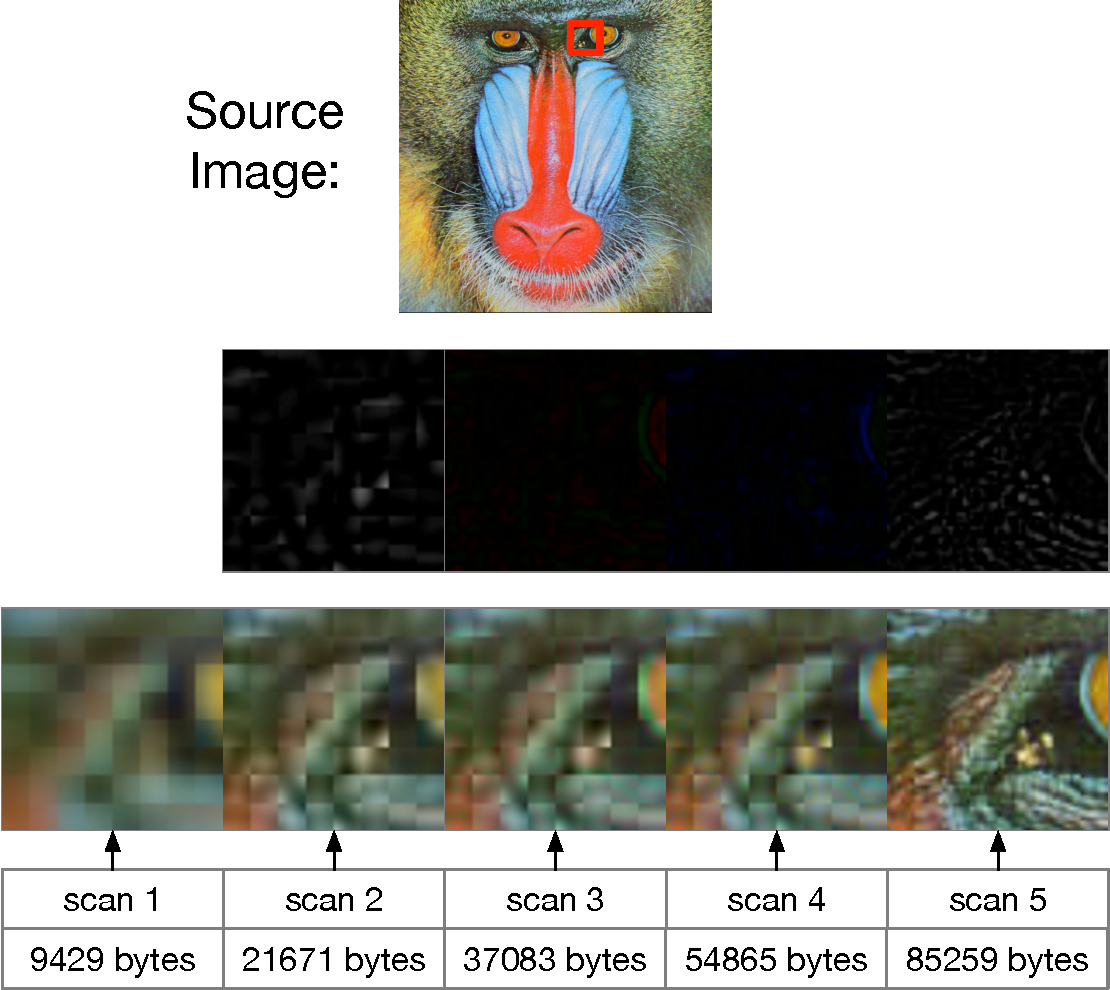
\includegraphics[width=\textwidth]{e2e_diagrams/progressive jpeg example.pdf}
    \caption{Example of an JPEG image with a progressive encoding (enlarged to show detail). Each image scan refines previous image data by including higher frequency coefficients. The image difference vs. the previous scan is show above each crop; cumulative number of bytes read are shown below.}
    \label{fig:progressivejpeg}
\end{figure}
Progressive JPEG achieves this property by arranging image data in multiple passes of increasing detail.
Concretely, the data layout groups image data roughly in frequency domain order, relying on the property that lower frequency coefficients tend to encode coarse image details first.
By transmitting (when reading or sending data) or rendering coarse details first, a lossy preview of the image can be generated before all the image data has been received or rendered.


Conveniently, this format can also be used to partition image data for lower resolution versions or previews~\cite{yan2017customizing}.
As an extreme example, using the first (DC) component of each $8\times8$ macroblock yields a subsampled image at 1/8th the original resolution.
By leveraging a quality metric, we can target resolutions in between 1/8th and the original resolution by mapping frequency coefficient groupings (called scans in JPEG) to target resolutions.
\autoref{fig:progressivejpeg} shows an example of how image detail increases as more scans of a progressive JPEG image are rendered.
We use this property explicitly to selectively load a fraction of the total image data when executing neural network inference at different image resolutions: lower resolutions require fewer progressive JPEG scans and fewer bytes of image data.
%Progressive JPEG typically results in images slightly smaller than images with data laid out in baseline or scanline order, due to the improved compressibility of grouped frequency coefficients.

\paragraph{Specializing Operator Implementations}
From a computation perspective, potential savings from reduced floating-point operations (FLOPs) materialize only when high compute utilization can be achieved across each resolution choice.
As the compute utilization of deep learning operators can be highly dependent on input shapes (e.g., resolution), operator implementations that are specialized for the range of resolutions are necessary.
Here, we leverage prior work on automatic tensor program optimization~\cite{chen2018learning, ragan2013halide} to generate resolution-specialized operator implementations while minimizing programmer effort.


%In this section, we provide further details on our motivation for dynamic multi-resolution support, and our choices for each of the requirements for its implementation.



\paragraph{Crop Sizes, Resolution, and Scale}
\label{sec:invariance}
\begin{figure}
    \centering
    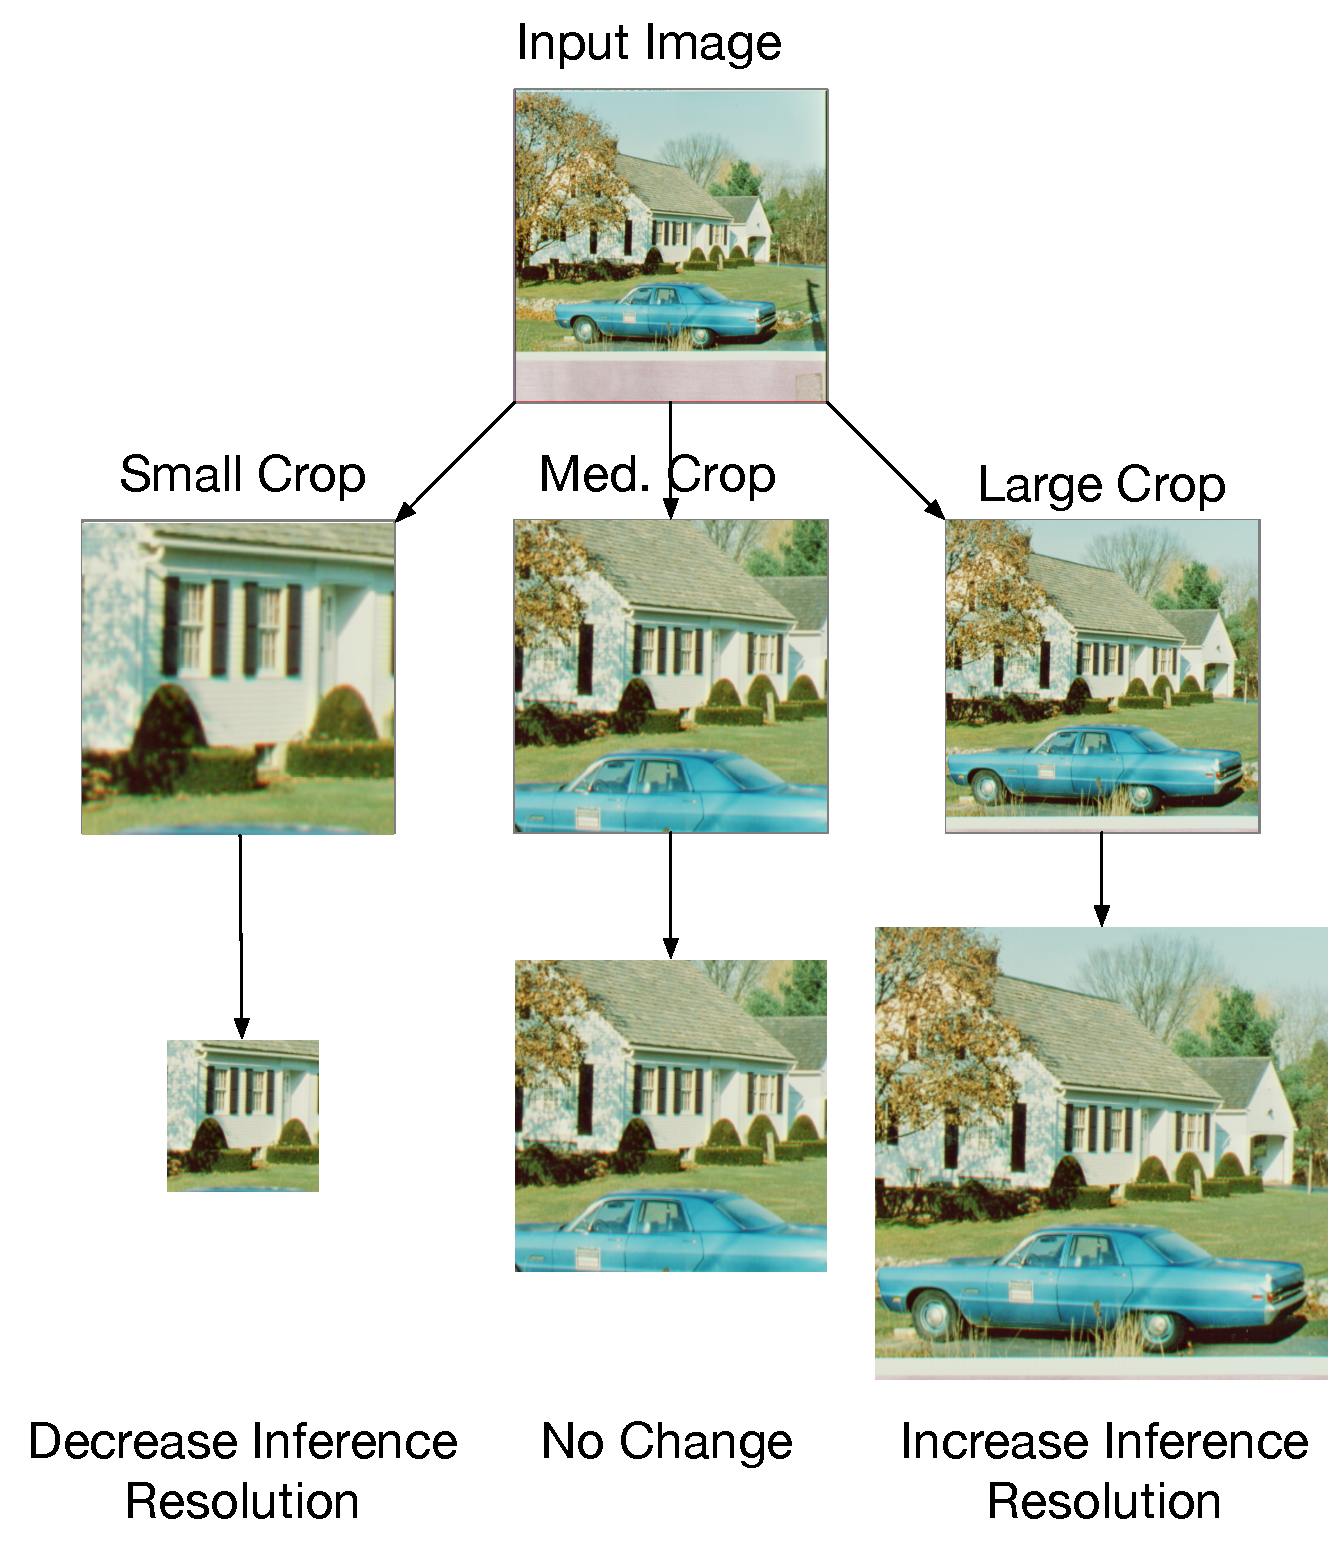
\includegraphics[width=\textwidth]{e2e_diagrams/scale variations.pdf}
\caption{Neural networks are sensitive to the apparent scale of objects. This apparent scale is determined by the image crop and the resolution used to evaluate the model. We show three different crops of the same image and the required change to the inference resolution required to match the object scales across the images.}
    \label{fig:cropexample}
\end{figure}
Efficient multiple-resolution support can be motivated by the lack of scale invariance (more formally, equivariance)~\cite{sosnovik2019scaleequivariant} in current computer vision models.
This issue stems from the fact that while convolution operators are translation equivariant, they are not scale equivariant~\cite{touvron2019fixing}.
\autoref{fig:cropexample} shows an example of how different crop sizes can present objects at different scales to neural networks, and the corresponding change to inference resolution required to compensate for scale differences.
The lack of scale equivariance results in models being sensitive to the distribution of object scales, and even with the typical remedy of data augmentation (e.g., in the form of random cropping), model performance can be improved by fine-tuning on a known scale distribution~\cite{touvron2019fixing}.
We characterize the impact of the issue of popular neural network architectures' \emph{lack} of scale invariance by evaluating model accuracy at several crop sizes---we will see that the favored resolutions for model inference heavily depends on the image crop size due to this phenomenon.
%We use the common practice of taking each crop from the center of the image, reporting the relative area of the entire image that is used.


\section{Choosing Image Resolution from Object Scale}
\begin{figure}
    \centering
    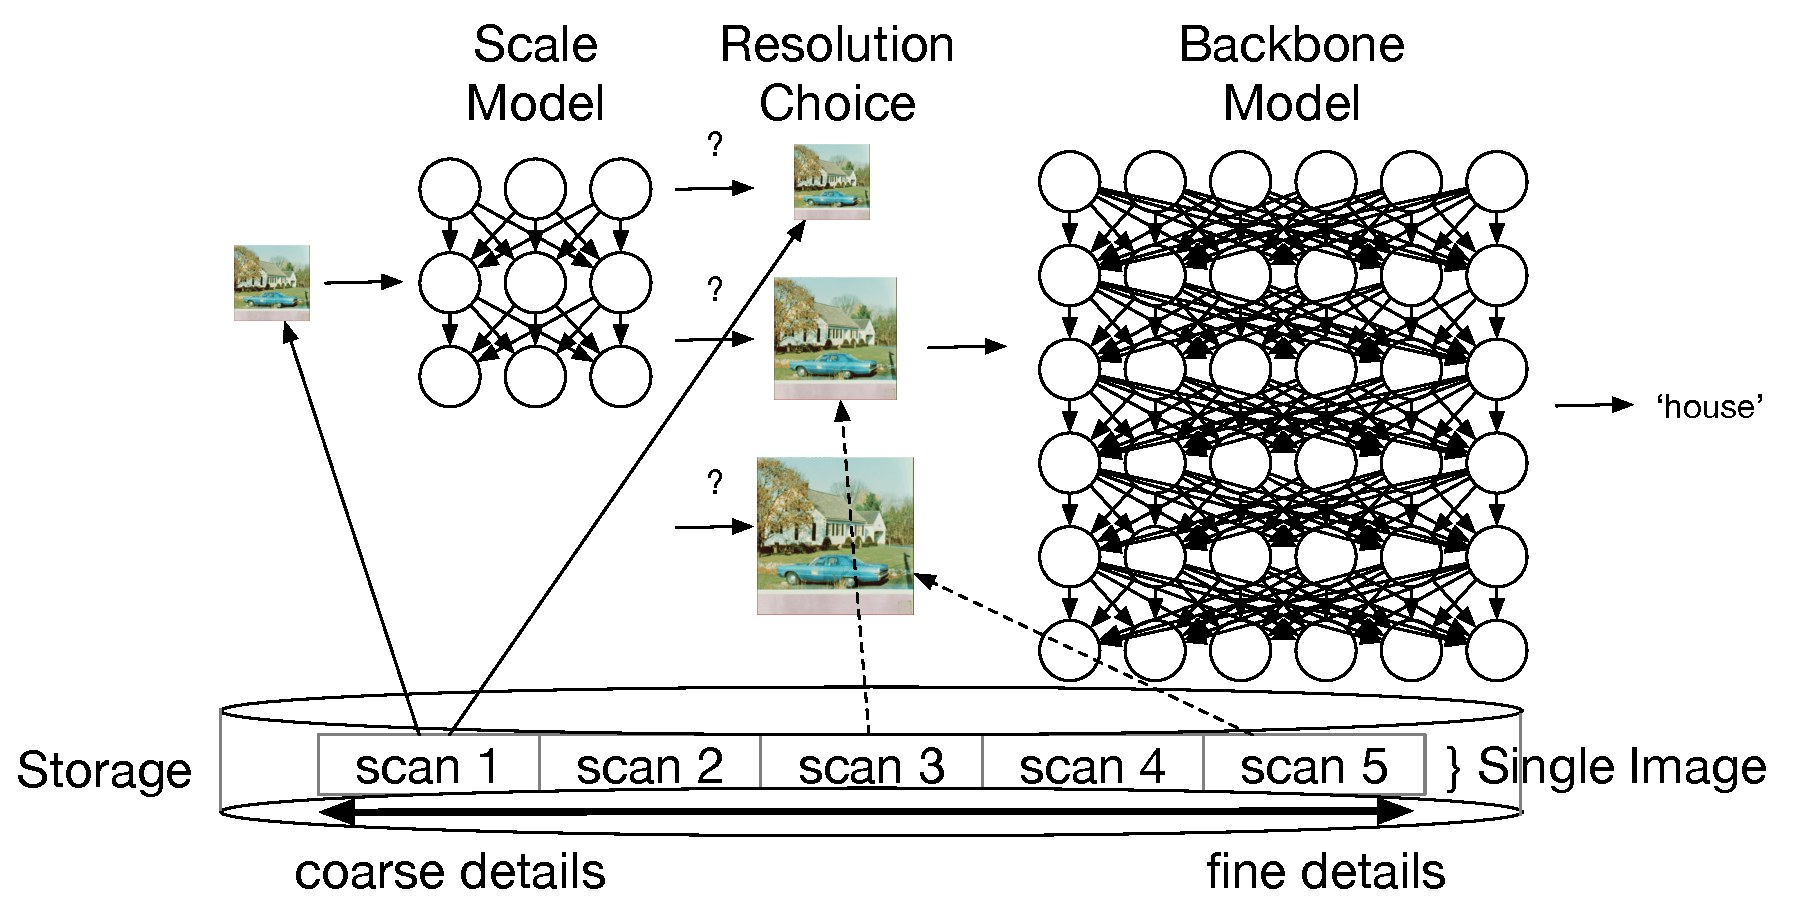
\includegraphics[width=\textwidth]{e2e_diagrams/overview figure.pdf}
    \caption{Example of a dynamic resolution system: images are stored with a progressive encoding that arranges each image as a sequence of scans. Low resolution images are first sent to a small scale model that predicts the best resolution for inference. If necessary, additional image data is read to to to generate the appropriate resolution for inference. }
    \label{fig:pipeline}
\end{figure}
We describe a simple way to leverage a multi-resolution enabled inference pipeline dynamically for object scales, by using two neural network models in sequence (\autoref{fig:pipeline}) such that resolution is chosen automatically.
We refer to the first model as the \emph{scale} model, as it roughly attempts to predict the appropriate scale for neural network inference.
We refer to the second model as the \emph{backbone} model; the backbone model performs the specified computer vision task a the chosen scale (resolution).
While this example two model pipeline introduces an additional control flow decision of which resolution to execute, this decision is at a coarse granularity (an entire image inference), we believe that this acceptable for inference workloads--especially those that typically run at batch size 1 (e.g., on CPUs).

\paragraph{Scale Model}
The scale is trained with a multilabel classification objective: it aims to predict whether a trained backbone model will be accurate at a given resolution for a given image.
At inference time, we select the resolution chosen by the scale model using the resolution with the highest predicted likelihood of making a correct prediction.
We find that as determining object scales does not require fine image details, the scale model can be lower in resolution (e.g., $112\times112$) relative to the backbone model without significantly sacrificing accuracy.
This reduction in resolution, combined with a choice of efficient model architecture minimizes the additional computational cost of the backbone model.

\paragraph{Backbone Model}
The backbone model for each dataset split (see \autoref{fig:crossval}) is trained as a standard classification model without additional modification.
Note that we do not train separate backbones for each resolution, instead relying on the input-shape agnostic operators of modern model architectures such as ResNet to reduce training costs.
%As current models typically are not shape-dependent, we train the backbone model at a single resolution but run it at multiple resolutions at inference time.
Running the model at a different resolution than it was trained with does not degrade accuracy, provided the object scales are matched.
However, the inference cost (in terms of FLOPs) increases nearly quadratically with the backbone model, as the computational complexity of convolution layers depends on the area of the input feature map.
True wall-clock scaling is slightly better, as higher compute complexity tends to also increase the utilization of hardware execution.
\begin{table}[]
    \centering
    \begin{tabular}{c|c|c|c}
       Model  & Resolution & GFLOPs & Accuracy  \\
    \hline
    ResNet-18 & $112\times112$ & 0.5 & 47.8\\ 
    ResNet-18 & $168\times168$ & 1.1 & 62.8\\ 
    ResNet-18 & $224\times224$ & 1.8 & 69.5\\ 
    ResNet-18 & $280\times280$ & 2.9 & \textbf{70.7}\\ 
    ResNet-18 & $336\times336$ & 4.2 & 70.1\\ 
    ResNet-18 & $392\times392$ & 5.8 & 69.4\\ 
    ResNet-18 & $448\times448$ & 7.3 & 68.9\\ 
    \end{tabular}
    \caption{Example of compute complexity scaling with input resolution (in billions of floating-point operations). Here, the accuracy values are obtained by performing inference on a model trained at $224\times224$ resolution, indicating the train-test resolution discrepancy~\cite{touvron2019fixing} where higher resolutions do not improve accuracy due to a scale mismatch. }
    \label{tab:my_label}
\end{table}

\paragraph{Scale Model Training}
The multilabel classification objective introduces the problem of another data split, as training a scale model required an already trained backbone model.
To leverage all available data when training the scale model, we train the scale model using a cross-validation style approach (\autoref{fig:crossval}).
Several backbone models are trained on disjoint parts of the training set, and the scale model is trained by alternating backbone models and the corresponding training sets.
For our evaluation, we train four different backbone models on 3/4ths of the ImageNet and Cars datasets, and train the scale model using the corresponding 1/4th split for each backbone.
When measuring end-to-end accuracy, we use a backbone trained on the full training set.

\begin{figure}
    \centering
    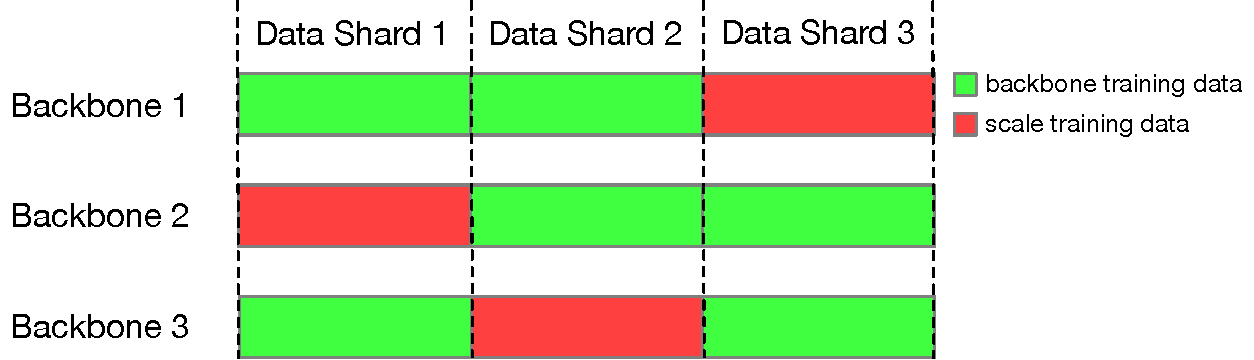
\includegraphics[width=\textwidth]{e2e_diagrams/cross val.pdf}
    \caption{Training a two model pipeline via a cross-validation style approach.
    %to train a scale model so that all training data can be used by both the backbone and scale model. Note that this requires training several backbone models to train a single scale model. At test-time, a backbone trained on the complete training set is used.
    }
    \label{fig:crossval}
\end{figure}


\section{Choosing How Much Data to Read For Each Resolution}
Given a quality metric, such as SSIM, we can use the quality metric to compare model accuracy against the amount of data read to establish curves
(\autoref{fig:calibration_imagenet_ssim}, \autoref{fig:calibration_cars_ssim}) for model accuracy and image quality for each resolution.
These curves can form the basis for a storage policy that chooses the amount of data to read for a given resolution requested by a computer vision model.
%If these curves have a clear knee or change in slope at some quality threshold, this presents a natural operating point, as further image data yields diminishing returns.
For our purposes, we use structural similarity, as it is more convenient to design a calibration algorithm that searches in the range [0.0, 1.0] than with PSNR where the value for ``perfect'' image quality goes to infinity.
Note that as the amount of data required for accurate inference is a data-dependent task, we pose this as a \emph{calibration} task, where a small amount of training data is reserved to tune quality thresholds determining when the amount of image data read is sufficient.

\paragraph{Datasets}
For storage calibration, we use two datasets chosen for their differences in resolution distribution and type of classification.
The first is the popular ImageNet dataset~\cite{russakovsky2015imagenet} comprising 1 million images of 1,000 object classes.
The second is the Stanford Cars dataset~\cite{krause20133d} comprising 16,185 images of 196 fine-grained object classes.
While the Cars dataset contains fewer images (with less than 1/100th the training set size of ImageNet), some are of considerably higher resolution than the ImageNet dataset, which yields potential differences when calibrating storage for inference at a given resolution.
The average dimensions of training images in the Cars dataset are $699\times482$ pixels while the average dimensions of images in the ImageNet dataset are $472\times405$ pixels.
\paragraph{Calibration Procedure}
To search for the minimal quality (SSIM threshold) that satisfies the accuracy target, we run binary search of over the SSIM interval [0.94, 1.0], and terminate the search after the step size falls below 0.0001, with the constraint that no more than 0.05\% accuracy is lost for each of the resolutions.
We use three different train/validation splits of Cars and ImageNet (shown as the different seeds in \autoref{fig:calibration_imagenet_ssim} and \autoref{fig:calibration_cars_ssim}). generated on the training set of the respective dataset, limiting the number of images used for calibration to 10,000 (to reduce the amount of computation required).
We use the median SSIM threshold found by this search for each resolution in our storage evaluation.

\autoref{fig:calibration_imagenet_ssim} and~ \autoref{fig:calibration_cars_ssim} show accuracy vs. the relative amount of data read (normalized to 1.0), averaged over a collection of images in the training set of ImageNet and Cars respectively.
Lower resolutions require less image data for the same SSIM value, but accuracy degrades more rapidly with respect to the amount of image data read.
Interestingly, while there is a general trend of accuracy increasing with the amount of image data read, the points at which the maximum accuracy is reached is not necessarily when all the image data is read.


We find substantial differences in the relationship between image quality and model accuracy for ImageNet vs. Cars.
These differences can be attributed to the respective distributions of image resolution the datasets, but another potential explanation is the difference in types of image features most important for different datasets.
Most immediately, the curves of accuracy vs. image read size appear to be shifted left for Cars vs. ImageNet: accuracy is better preserved even when images are loaded at low fidelity for Cars.
If ImageNet favors fine-grained texture details while Cars favors abstract shapes, this can explain the different image quality requirements.

One trend common to both datasets is that higher image resolutions often required lower image quality (when compared to the ground truth resized image) to maintain model accuracy.
This trend is surprising as intuitively, one might expect a benefit of higher input resolution to be the inclusion of details lost after resizing to lower resolutions.
In fact, this trend is pronounced enough that maintaining accuracy at higher inference resolutions may require less image data to be read than for inference at lower resolutions.
For Cars, minimal accuracy losses were observed at higher resolutions even when just over half the image data was read.
On ImageNet, this effect was less pronounced, with over 80-90\% of image data required to minimize accuracy loss at higher resolutions.
%We also note that the absolute highest accuracy obtained for each resolution does not necessarily occur when all of the available image data is used; this may be because omitting image data helps to mitigate the effects of overfitting to fine image details.


%\begin{figure}
%    \centering
%    \includegraphics{placeholder.png}
%    \caption{Comparison of PSNR and Structural Similarity at a Single Resolution}
%
%    \label{fig:my_label}
%\end{figure}


\begin{figure*}
    \centering
    \begin{tabular}{@{}c@{}}
    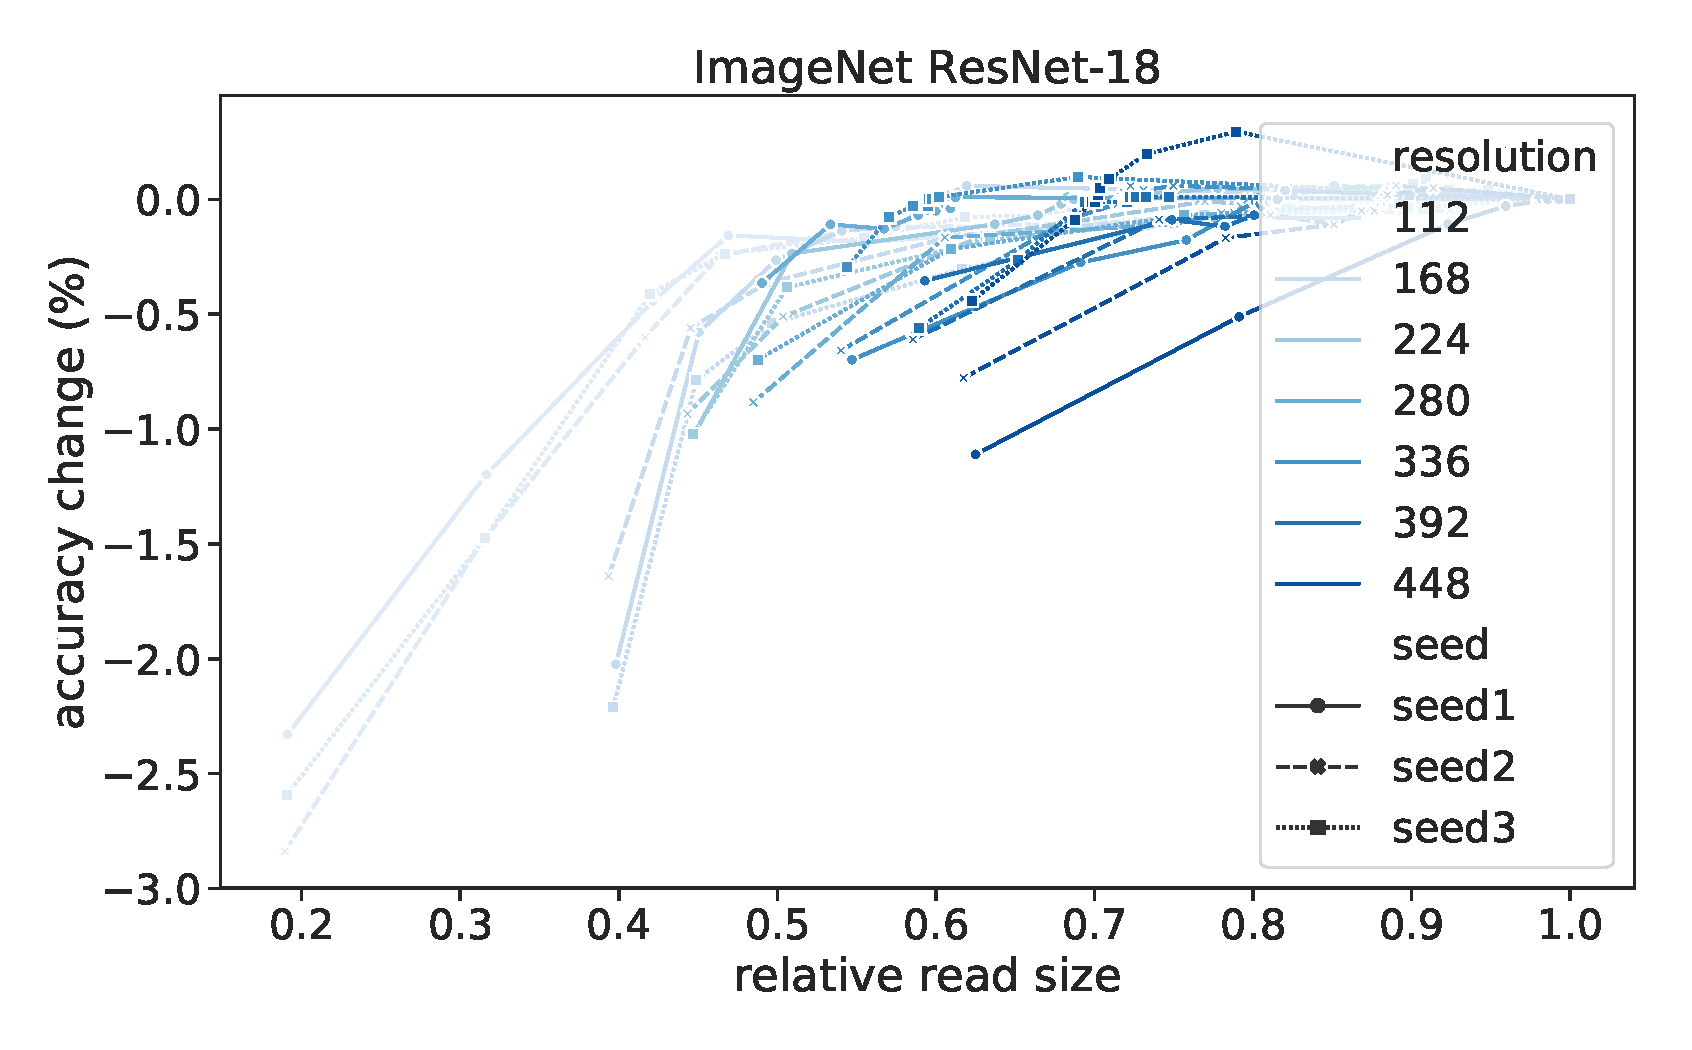
\includegraphics[width=\textwidth]{e2e_figures/calibration_imagenetresnet18.pdf}\\
    \small (a)
    \end{tabular}
    \begin{tabular}{@{}c@{}}
    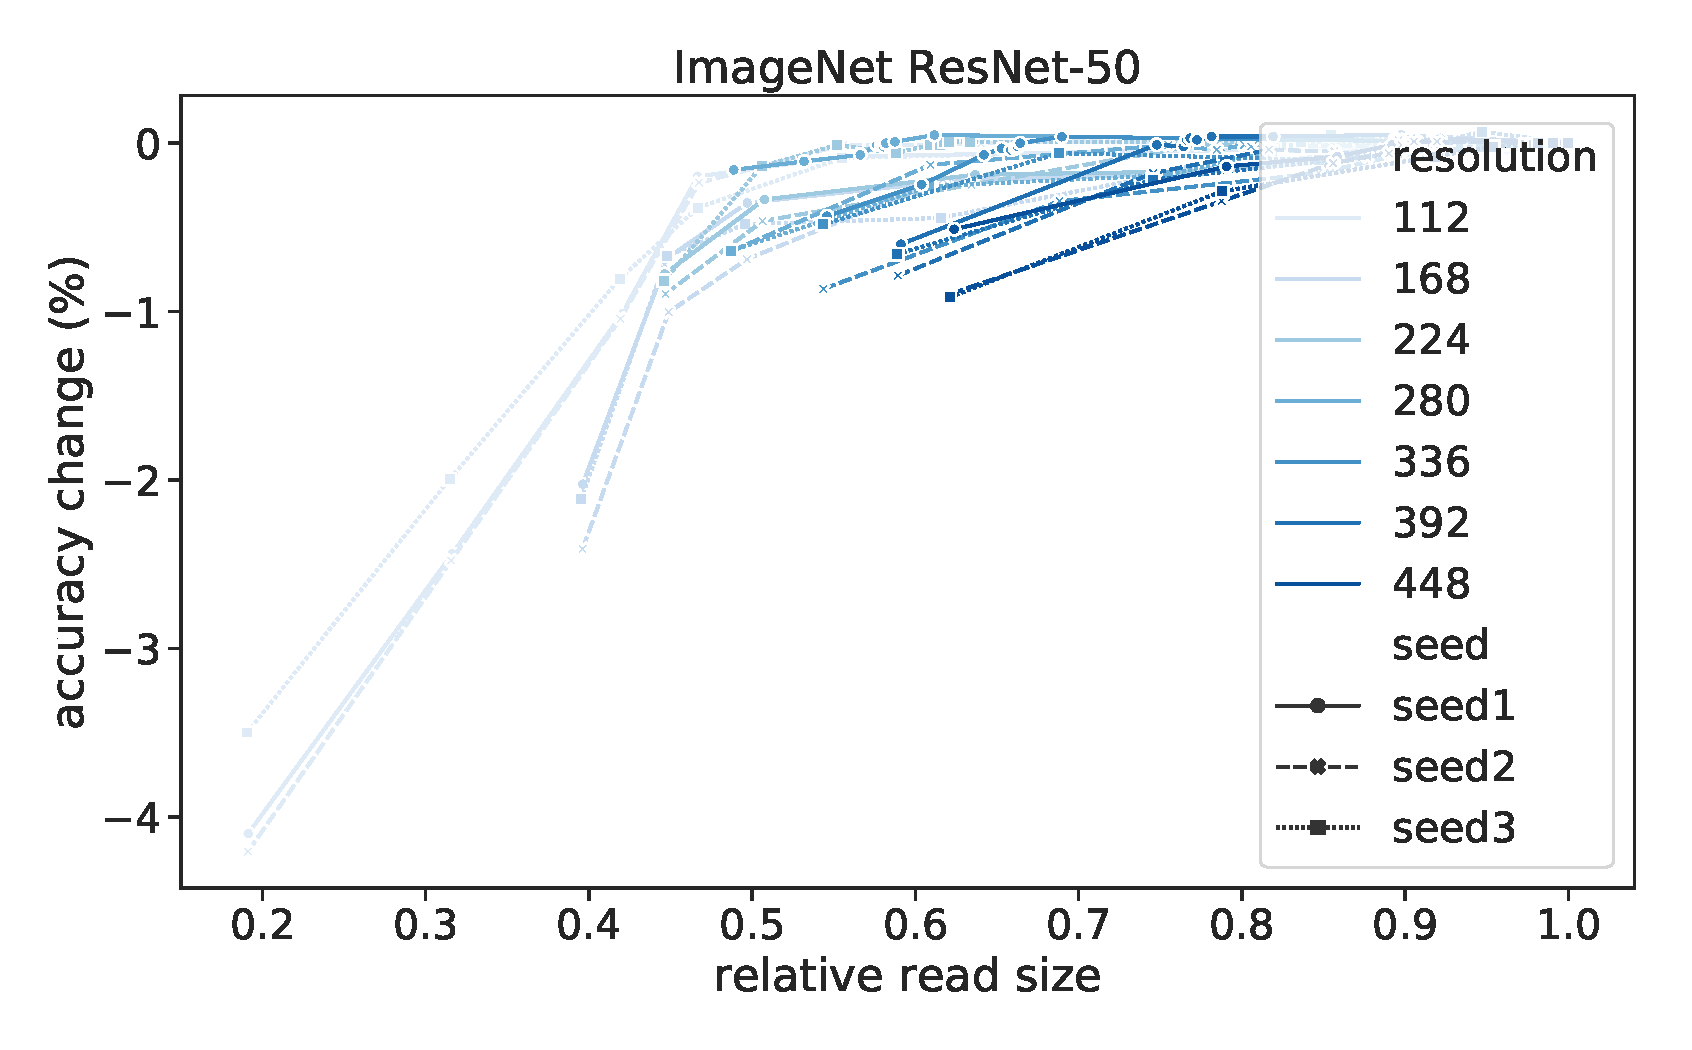
\includegraphics[width=\textwidth]{e2e_figures/calibration_imagenetresnet50.pdf}\\
    \small (b)
    \end{tabular}
    \caption{Storage calibration: relative top1 accuracy change of ResNet-50 and ResNet-18 on ImageNet at different resolutions with varying amounts of image data read vs. reading all image data at each resolution. 
    %The three seeds indicate different models trained and evaluated with different train/test splits. 
    %The amount of image data read (1.0 indicates the entire file is read) is determined by sweeping a range of SSIM values and progressive JPEG scans. Lower resolutions require less image data for the same SSIM value, but accuracy degrades more rapidly with respect to the amount of image data read.
    }
    
    \label{fig:calibration_imagenet_ssim}
\end{figure*}
\begin{figure*}
    \centering
    \begin{tabular}{@{}c@{}}
    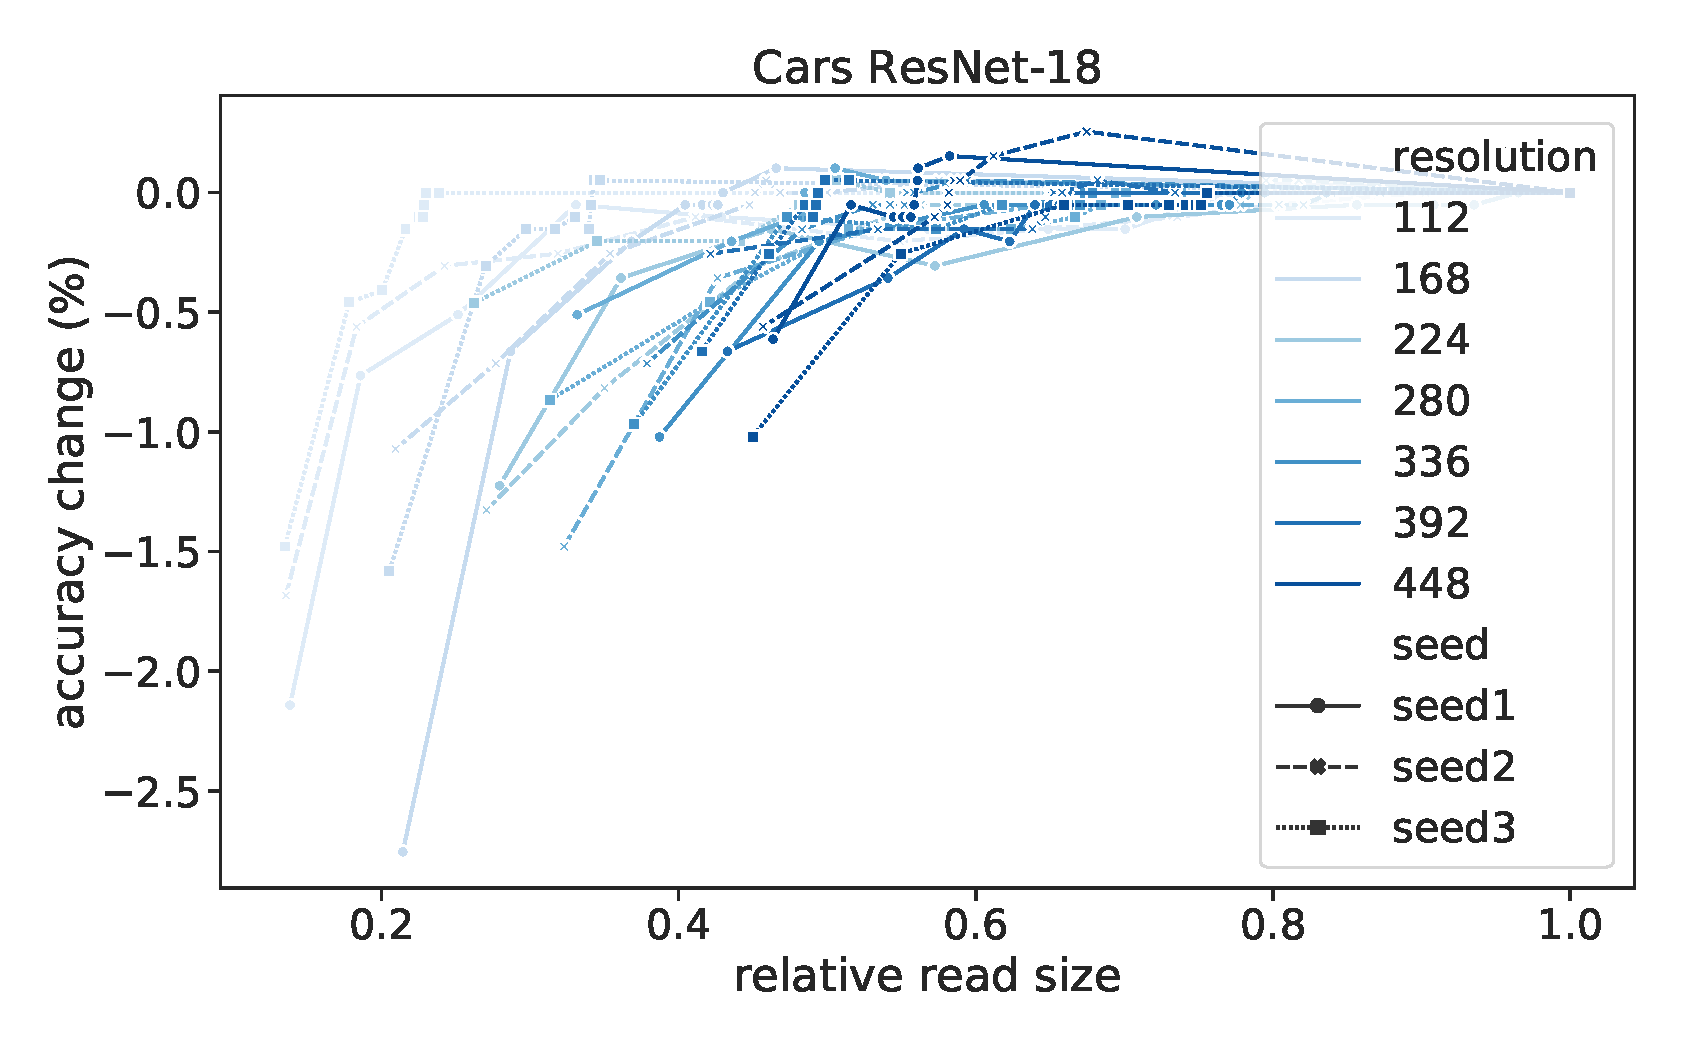
\includegraphics[width=\textwidth]{e2e_figures/calibration_carsresnet18.pdf}\\
    \small (a)
    \end{tabular}
    \begin{tabular}{@{}c@{}}
    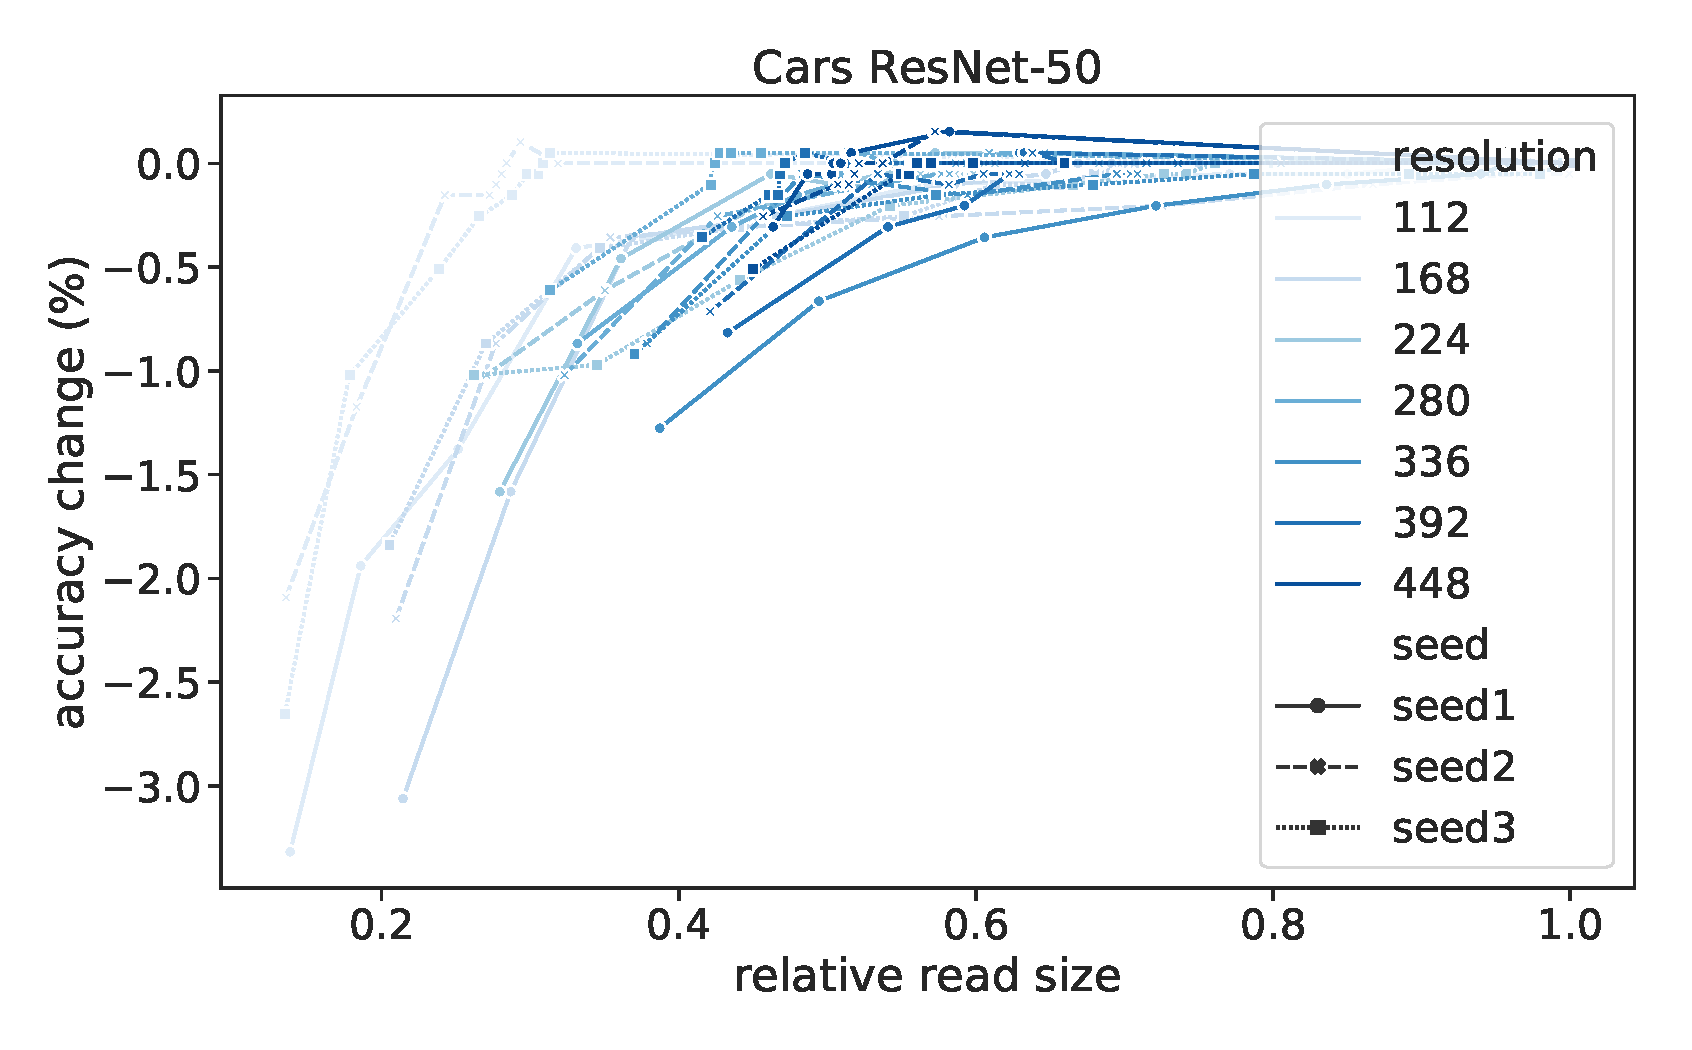
\includegraphics[width=\textwidth]{e2e_figures/calibration_carsresnet50.pdf}\\
    \small (b)
    \end{tabular}
    \caption{Storage calibration: relative top1 accuracy change of ResNet-18 and ResNet-50 on Stanford Cars at different resolutions with varying amounts of image data read.}
    \label{fig:calibration_cars_ssim}
\end{figure*}

\section{Maximizing Hardware Utilization for Each Resolution}
\begin{figure}[t]
    \centering
    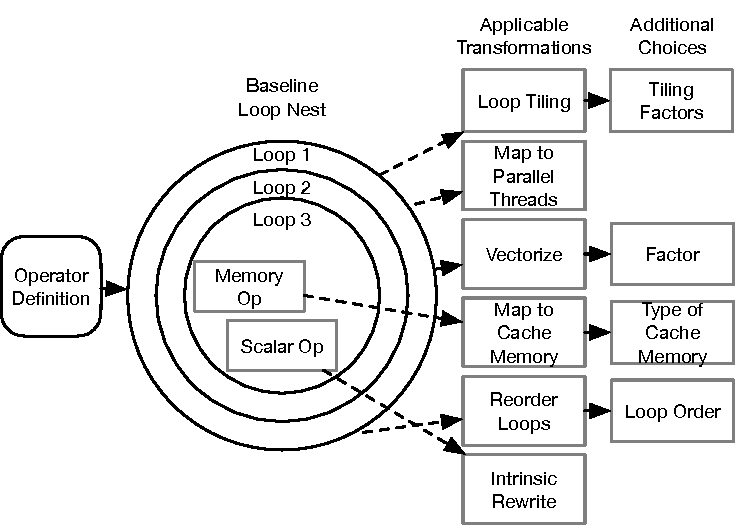
\includegraphics[width=\textwidth]{e2e_diagrams/searchspace.pdf}
    \caption{Example of the search space of a deep learning operator such as 2D convolution. We use a predefined search space to optimize the implementation of the model for different CPUs at different resolutions.}
    \label{fig:searchspace}
\end{figure}
Our goal with respect to compute kernels is to find the optimal implementation for every resolution, ideally preserving hardware utilization across all resolutions.
Common computationally intensive operators for computer vision models such as 2D convolution typically require highly specialized implementations on modern hardware such as GPGPUs or even CPUs with wide vector instruction sets.
As these specialized implementations depend on hardware implementation details such as the organization and size of the compute units (e.g., CUDA cores) and memory hierarchy (e.g., Shared/Scratchpad memory, caches, and global DRAM), they are also highly dependent on input sizes and data layouts.
These dependencies mean that implementations are also highly sensitive input shapes for each operator, which are dependent on the input resolution to a neural network model.
While it is possible to manually craft implementations for each neural model and resolution, the combination of the two pose a tedious engineering challenge.
Here, we leverage prior work on automatic compiler optimizations~\cite{chen2018learning} for shape-specific deep learning kernels to generate a specialized implementation for each resolution.
With the use of autotuning, we characterize the throughput gap (\autoref{fig:tuning}) between high and low resolution inference stemming from decreasing hardware utilization, especially among library implementations that may be overfitted to specific resolutions.

Operator tuning searches a wide space of possible parameter choices for the highest performing combination.
\autoref{fig:searchspace} shows an abstract example of the choices for a deep learning operator.
These parameter choices include loop tiling factors, data layouts, and loop orderings among others.
This search can be viewed as a black-box optimization problem (in fact, the underlying code generator and hardware comprise multiple black boxes), and is performed by directly measuring running times of each implementation on hardware.
We note that this process can be expensive (on the order of hours per-neural network resolution and model), but this cost can be amortized quickly with many neural network inferences.
As we target inference pipelines, we focus on optimizations for commodity x86 CPUs, although the approach is general across all hardware devices such as GPGPUS\footnote{A highly related problem on GPGPUs is the issue of sustaining hardware utilization at batch size 1, where the may not be enough computation to "fill the machine'' per inference example.}.



\section{Evaluation}
We cover several aspects of efficiency in our evaluation, starting with optimizing utilization and wallclock time latency through operator autotuning for each resolution in \autoref{sec:tuning}.
Next, we move to the relationship between inference resolution, image crop sizes, and computational cost in \autoref{sec:accflops}.
Finally, we cover the impact of storage calibration for reducing the amount of read data necessary for each inference resolution in \autoref{sec:storage}.

\subsection{Closing the Throughput Gap for Each Resolution}
\label{sec:tuning}
\begin{figure*}[t]
    \centering
    \begin{tabular}{@{}c@{}}
    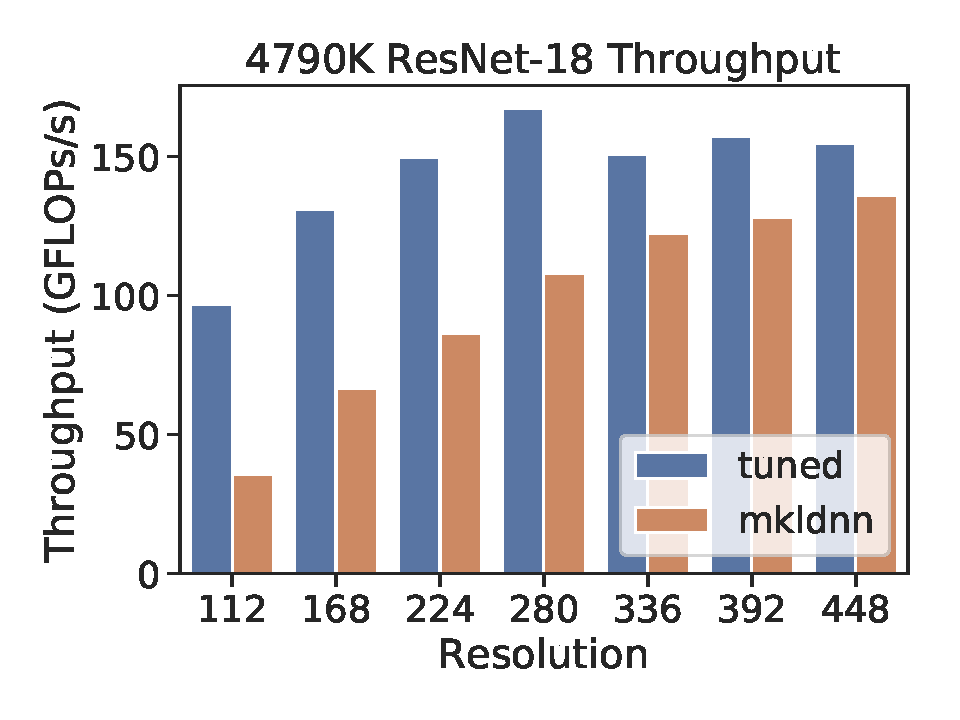
\includegraphics[width=0.45\textwidth]{e2e_figures/4790K_perf_data_resnet18.pdf}\\
    \small (a)
    \end{tabular}
    \begin{tabular}{@{}c@{}}
    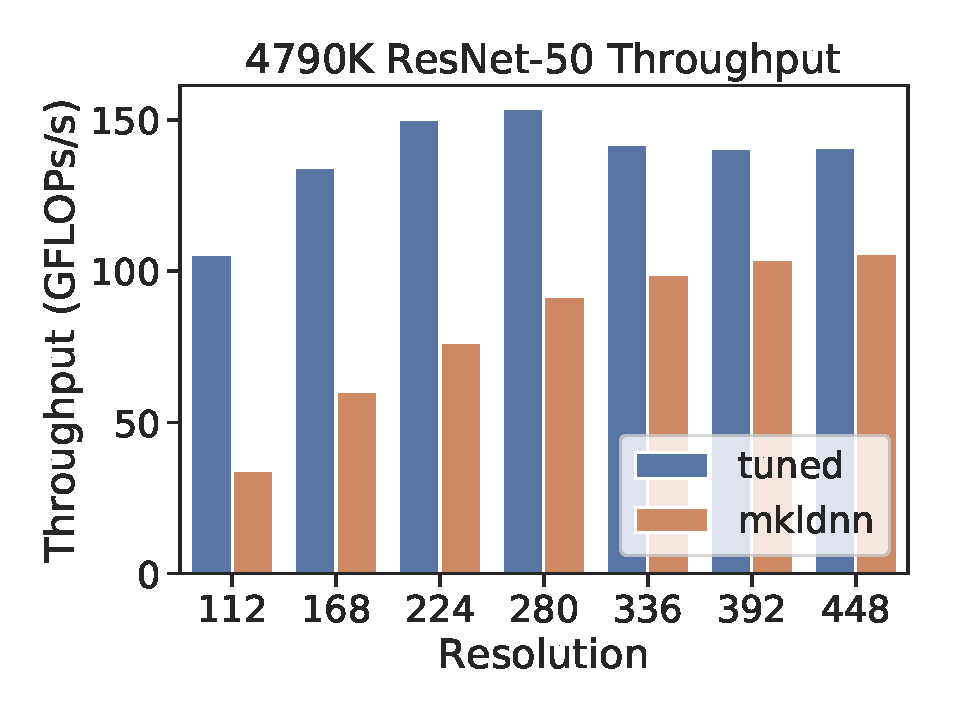
\includegraphics[width=0.45\textwidth]{e2e_figures/4790K_perf_data_resnet50.pdf}\\
    \small (b)
    \end{tabular}
    \begin{tabular}{@{}c@{}}
    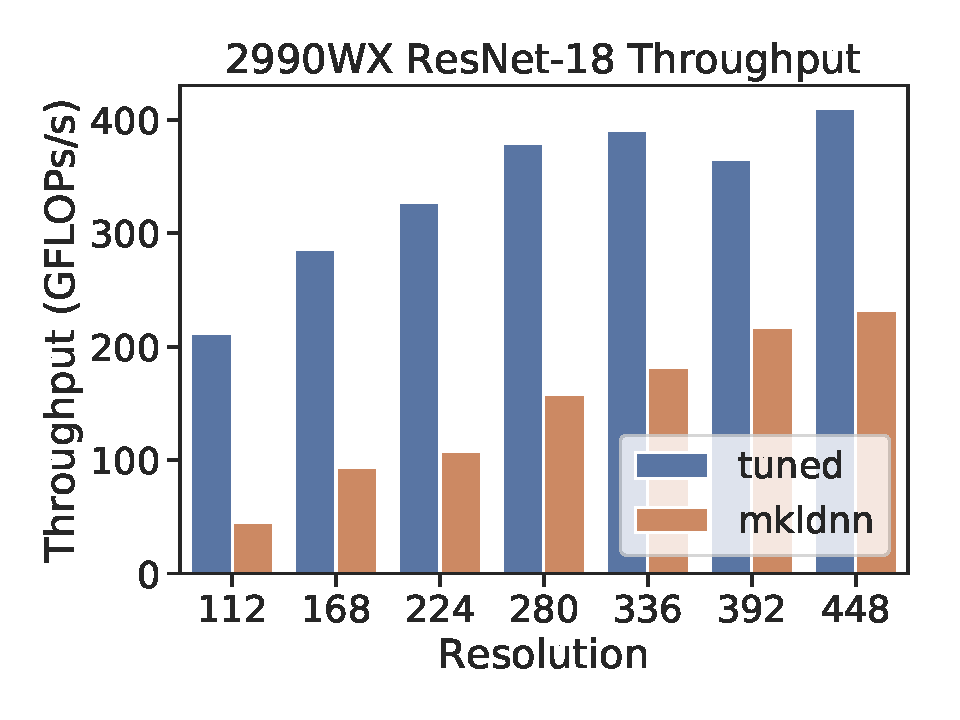
\includegraphics[width=0.45\textwidth]{e2e_figures/2990WX_perf_data_resnet18.pdf}\\
    \small (c)
    \end{tabular}
    \begin{tabular}{@{}c@{}}
    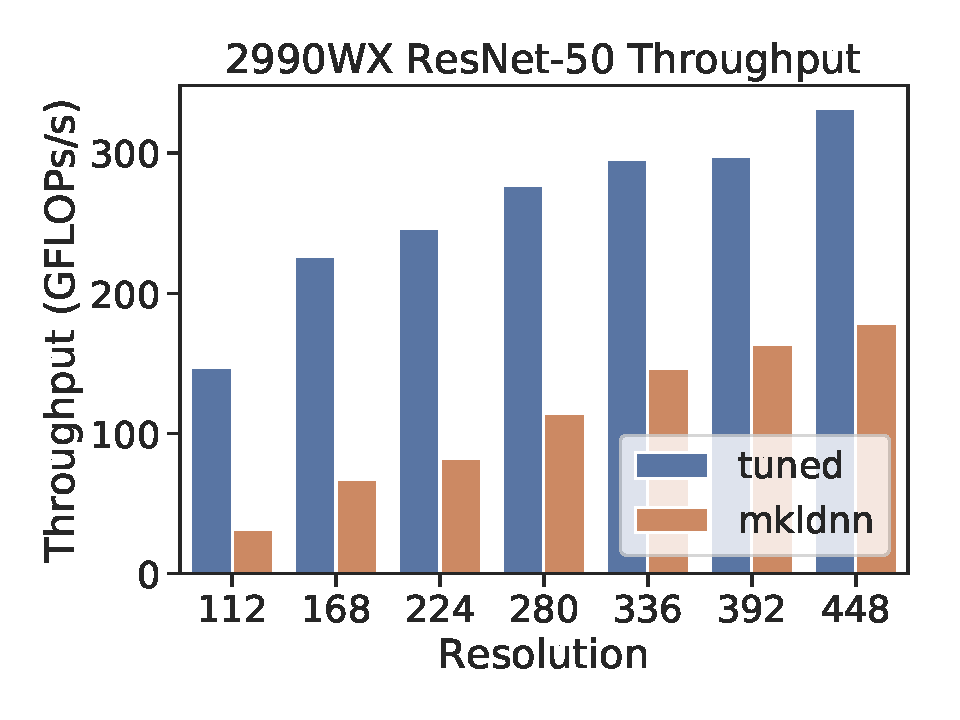
\includegraphics[width=0.45\textwidth]{e2e_figures/2990WX_perf_data_resnet50.pdf}\\
    \small (d)
    \end{tabular}
    \caption{Throughput of ResNet-18 and ResNet-50 at different resolutions (plotted according to GFLOPs/s) using the Intel MKLDNN Library compared with a tuned implementation for each resolution measured on Intel 4790K and AMD 2990WX processors. Tuning better sustains throughput at lower resolutions.}
    \label{fig:tuning}
\end{figure*}
\autoref{fig:tuning} compares the inference time for ResNet-18 and ResNet-50 using a library implementation (Intel MKLDNN) and using a tuned version for each resolution.
Here, we consider the typical inference scenario of batch size one.
While there is an absolute improvement in performance, we emphasize that the tuned implementations achieve better throughput (even compared to tuned high resolution kernels) for lower resolutions that have fewer operations.
Here, the challenge is to keep the utilization of the hardware high even when the model contains roughly $\frac{1}{16}$th the number of operations.
We observe the same effect on both the AMD 2990WX and 4790K (\autoref{fig:tuning} (a) vs. (c) and (b) vs. (d)).
Ideally, the bar plot of throughput would be flat across all the resolutions, indicating perfect scaling and identical hardware utilization across each of the resolutions.

We find that the scaling differences between specialized and library implementations are large, especially when comparing the two extremes in image resolution.
%The further a given approach's scaling curve (line) is from the origin (i.e., the ideal where 0 GFLOPs should incur 0 milliseconds of latency), the greater the constant-factor penalty for lower resolution inference.
Concretely, this translates into a speedup of only $3.9\times$ and $4.9\times$ when comparing inference at $448\times448$ to $112\times112$ on 4790K for ResNet-18 and ResNet-50 respectively.
Note that ideal scaling with GFLOPs in each case is $15.0\times$ for ResNet-18 and $15.2\times$ for ResNet-50.
With tuning, more of the ideal scaling in each case is recovered
as $9.4\times$ and $11.4\times$ speedups are achieved when switching from $448\times448$ to $112\times112$ resolution.
This pattern is more pronounced on AMD 2990WX (which likely has less targeted optimizations in MKLDNN), where the untuned scaling from $448\times448$ to $112\times112$ is $2.9\times$ and $2.7\times$ vs. $7.7\times$ and $6.7\times$ for the tuned approach on ResNet-18 and ResNet-50 respectively.
Even when comparing higher resolutions, the impact of imperfect scaling is measurable: $3.2\times$ speedup is achieved when switching from ResNet-18 @ $448\times448$ to $224\times224$ using tuned kernels and only $1.9\times$ using MKLDNN on 2990WX.
The results are similar on 4790K: (MKLDNN $2.5\times$ vs. $3.9\times$ tuned on 4790K).
For lower resolution inference, we find the ideal operating point to be $168\times168$ due to the lower compute complexity while most of the throughput of higher resolutions is also attainable with tuning (68-70\% on 2990WX, and 85-95\% on 4790K). 

\subsection{Accuracy vs. FLOPs}
\label{sec:accflops}
\begin{figure*}[t]
    \centering
    \begin{tabular}{@{}c@{}}
    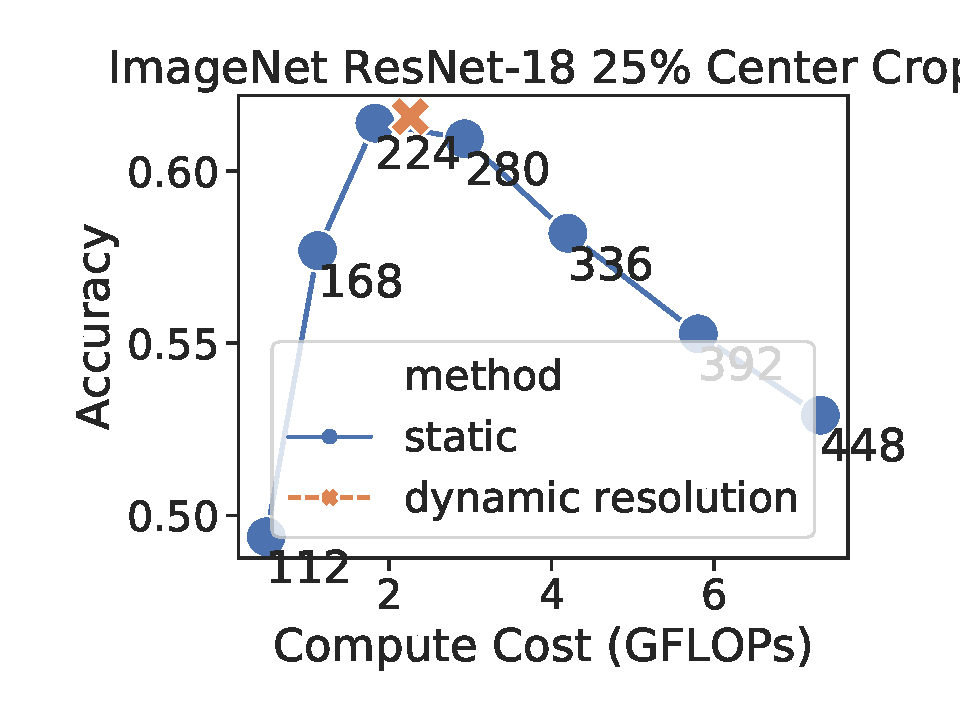
\includegraphics[width=0.45\textwidth]{e2e_figures/imagenet_resnet18_25_center.pdf} \\
    \small (a)
    \end{tabular}
    %\begin{tabular}{@{}c@{}}
    %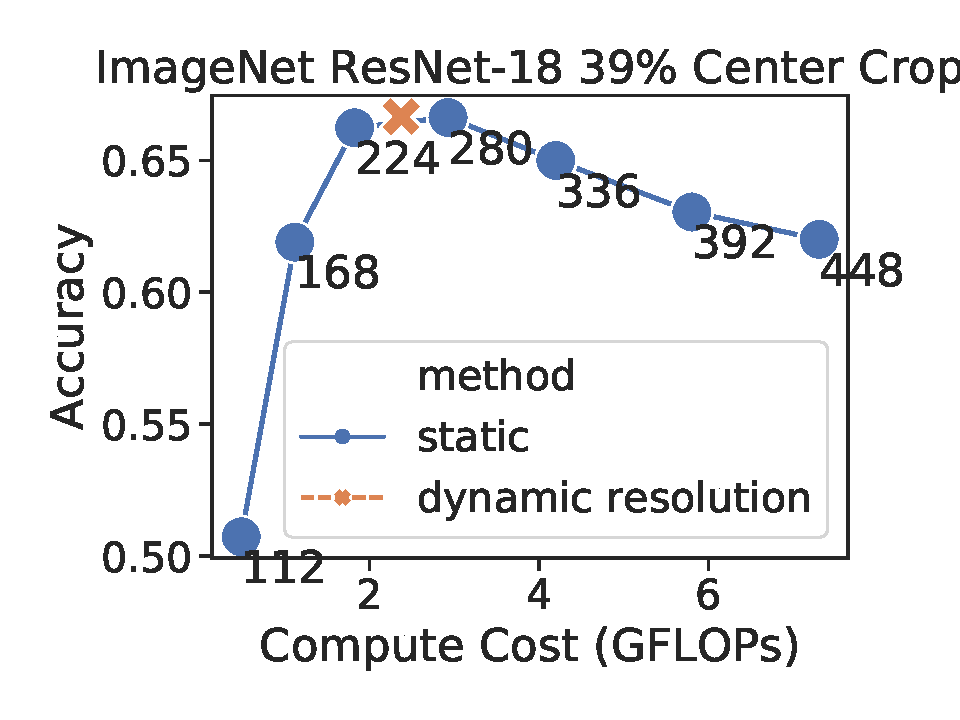
\includegraphics[width=0.195\textwidth]{asplos20-latex-template/figures/imagenet_resnet18_39_center.pdf} \\
    %\small (b)
    %\end{tabular}
    \begin{tabular}{@{}c@{}}
    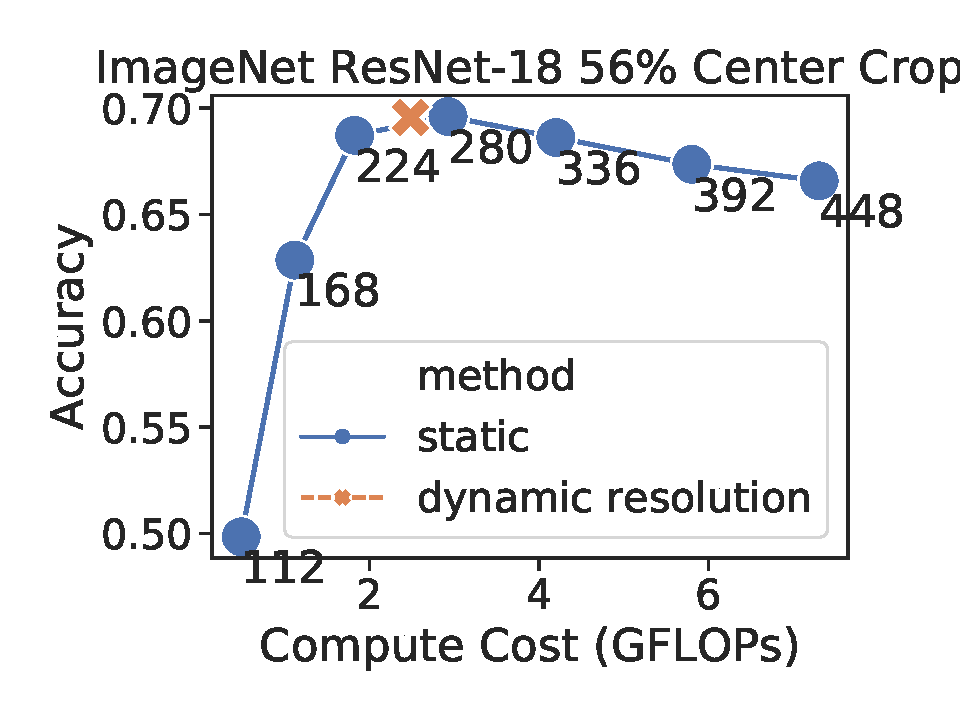
\includegraphics[width=0.45\textwidth]{e2e_figures/imagenet_resnet18_56_center.pdf} \\
    \small (b)
    \end{tabular}
    \begin{tabular}{@{}c@{}}
    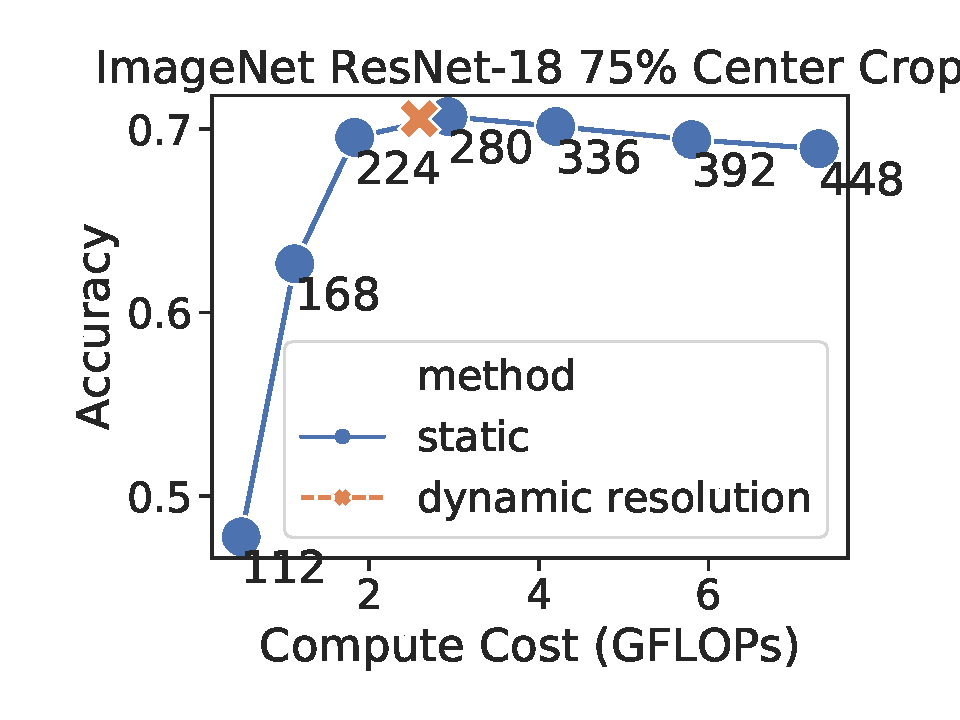
\includegraphics[width=0.45\textwidth]{e2e_figures/imagenet_resnet18_default_center.pdf} \\
    \small (c)
    \end{tabular}
    \begin{tabular}{@{}c@{}}
    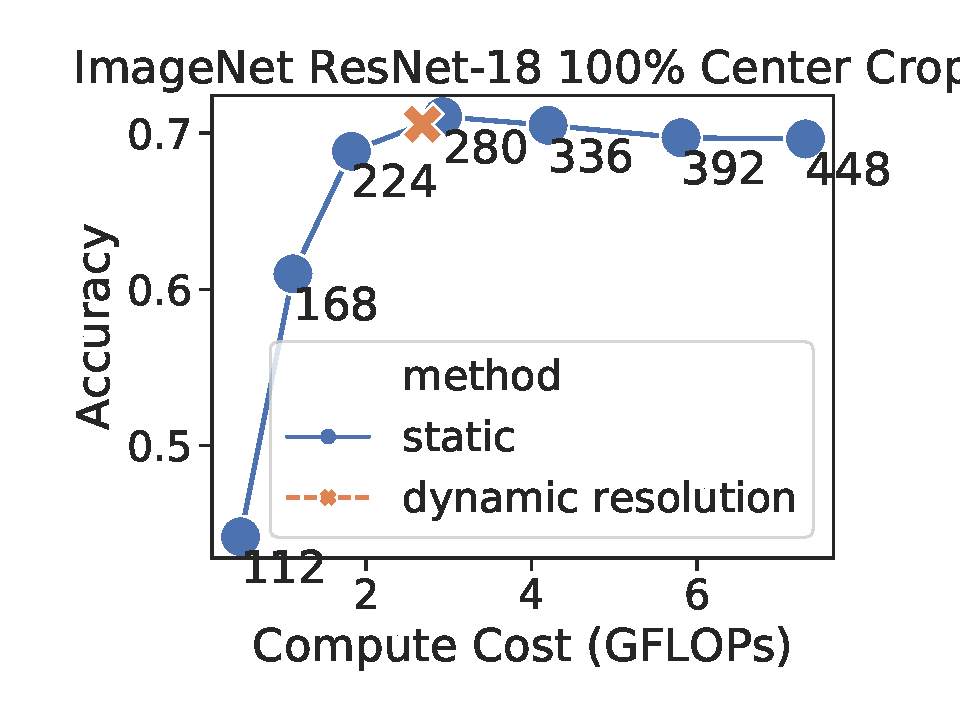
\includegraphics[width=0.45\textwidth]{e2e_figures/imagenet_resnet18_full_center.pdf} \\
    \small (d)
    \end{tabular}
    \begin{tabular}{@{}c@{}}
    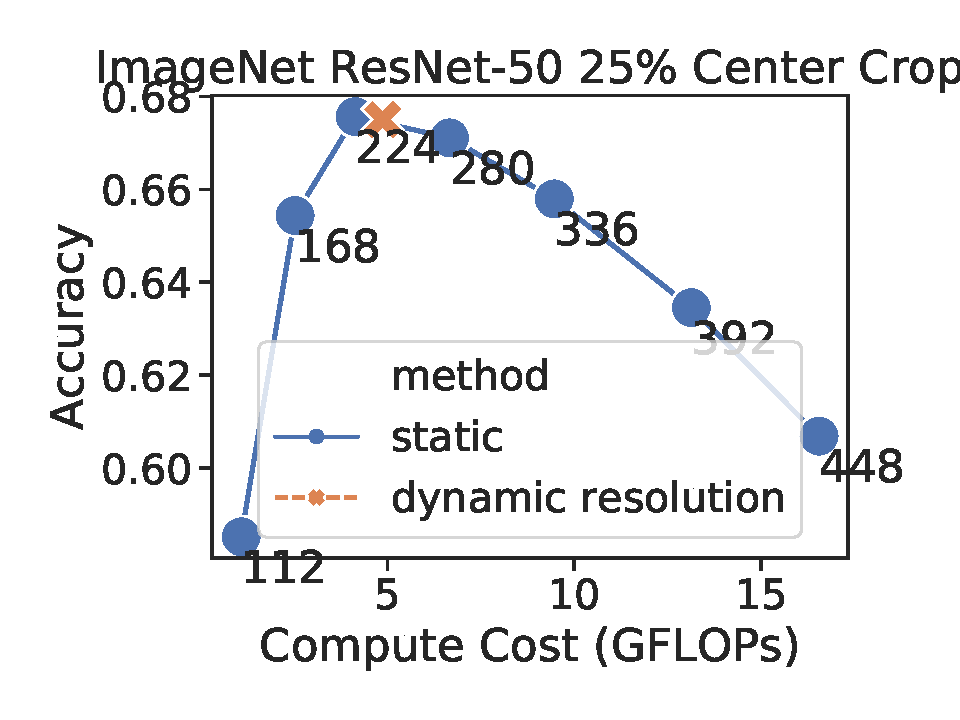
\includegraphics[width=0.45\textwidth]{e2e_figures/imagenet_resnet50_25_center.pdf} \\
    \small (e)
    \end{tabular}
    %\begin{tabular}{@{}c@{}}
    %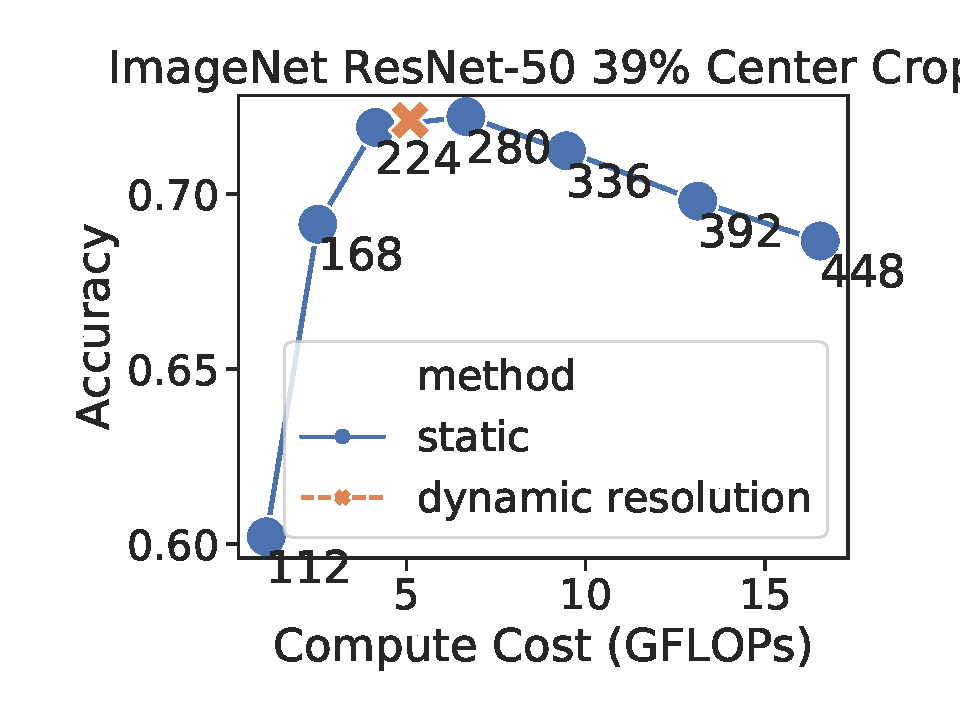
\includegraphics[width=0.195\textwidth]{asplos20-latex-template/figures/imagenet_resnet50_39_center.pdf} \\
    %\small (g)
    %\end{tabular}
    \begin{tabular}{@{}c@{}}
    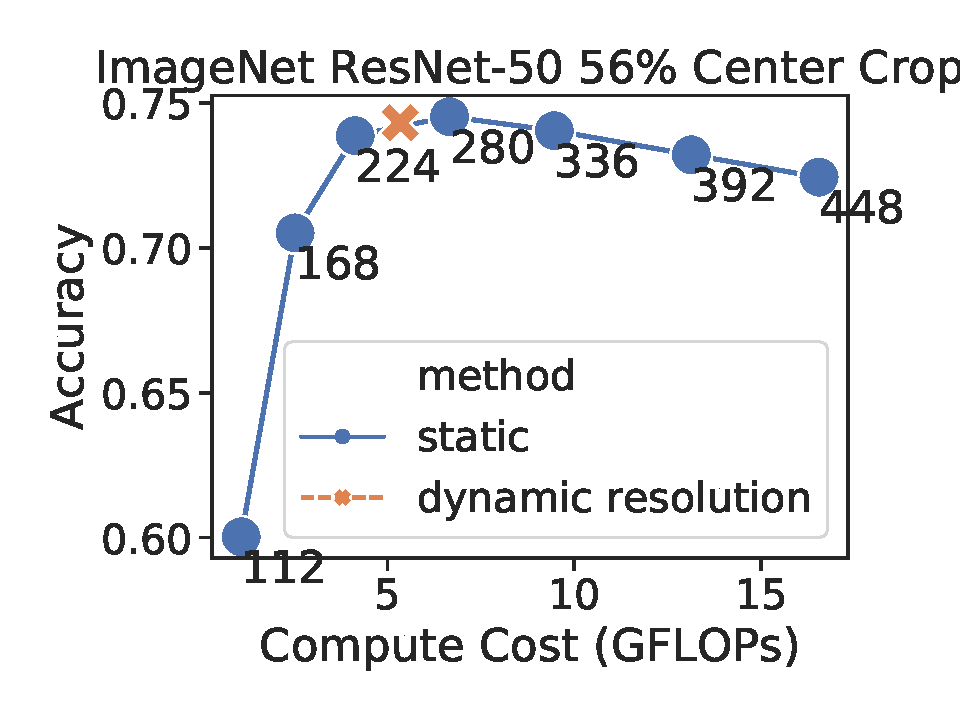
\includegraphics[width=0.45\textwidth]{e2e_figures/imagenet_resnet50_56_center.pdf} \\
    \small (f)
    \end{tabular}
    \begin{tabular}{@{}c@{}}
    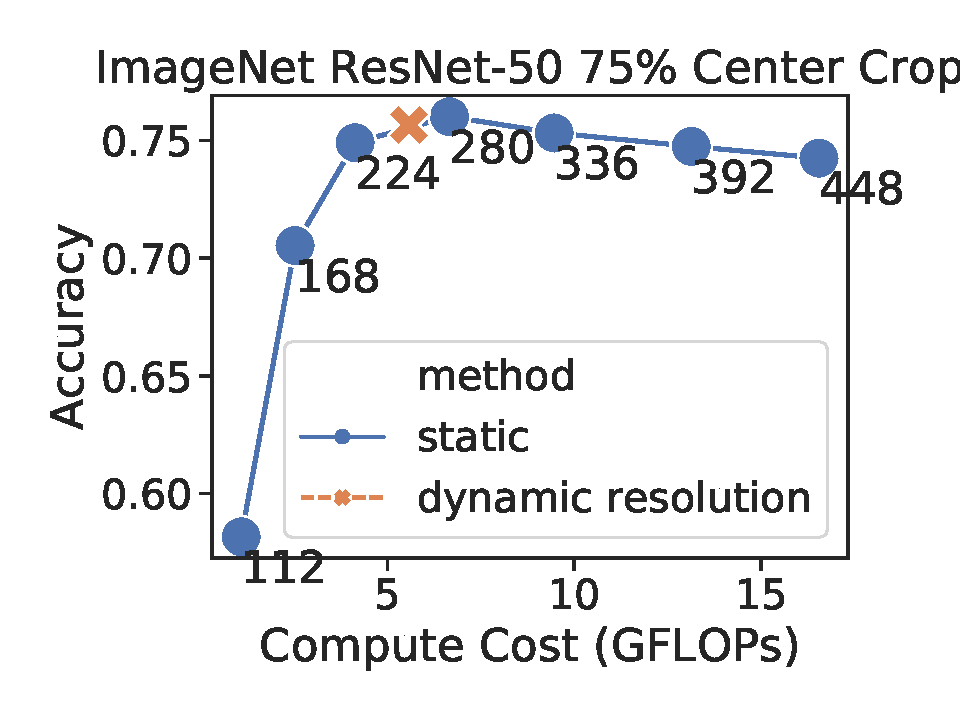
\includegraphics[width=0.45\textwidth]{e2e_figures/imagenet_resnet50_default_center.pdf} \\
    \small (g)
    \end{tabular}
    \begin{tabular}{@{}c@{}}
    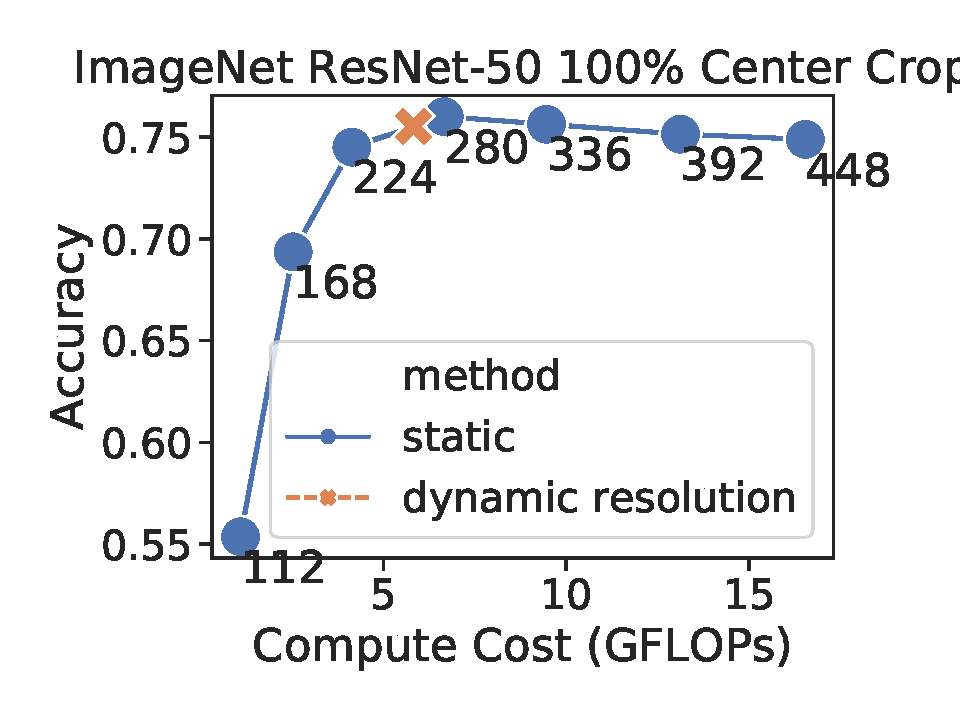
\includegraphics[width=0.45\textwidth]{e2e_figures/imagenet_resnet50_full_center.pdf} \\
    \small (h)
    \end{tabular}
    \caption{Accuracy vs. FLOPs comparison with static and dynamic resolution approaches using ResNet-18 (a-d)and 50 (e-h) on ImageNet. Crop sizes increase from left to right from 25\% on the left to 100\% on the right. Smaller crops favor lower resolutions more, while larger crops favor higher resolutions due to the models' dependence on object scale. The dynamic resolution approach operates at nearly the apex of every pareto curve, without hardcoding resolution.}
    \label{fig:accflops_resnet}
\end{figure*}
\begin{figure*}[t]
    \centering
    \begin{tabular}{@{}c@{}}
    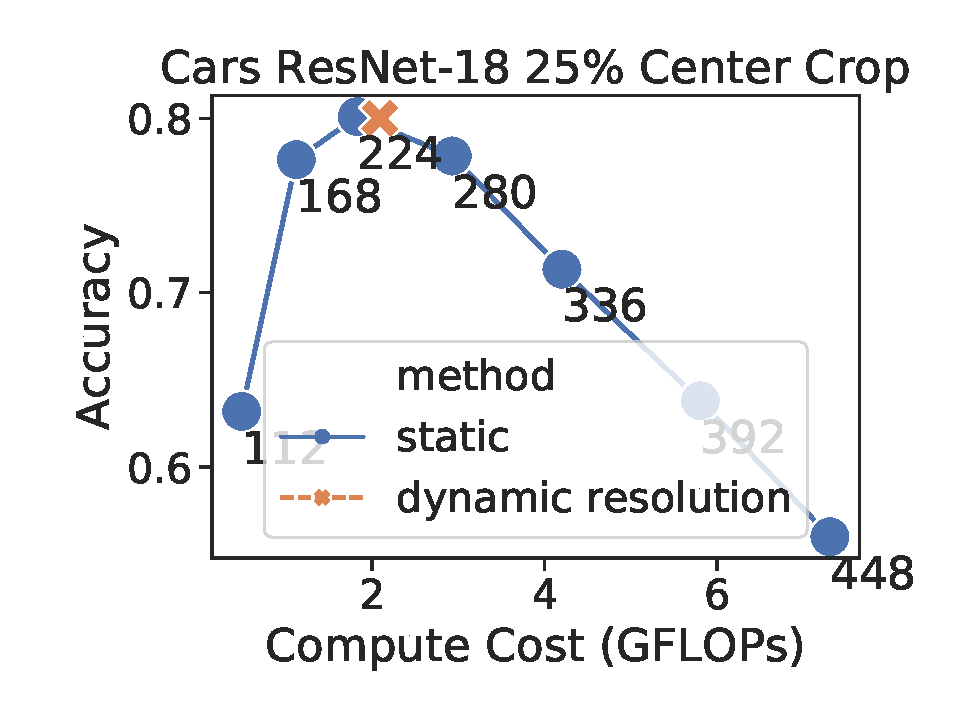
\includegraphics[width=0.45\textwidth]{e2e_figures/cars_resnet18_25_center.pdf} \\
    \small (a)
    \end{tabular}
    %\begin{tabular}{@{}c@{}}
    %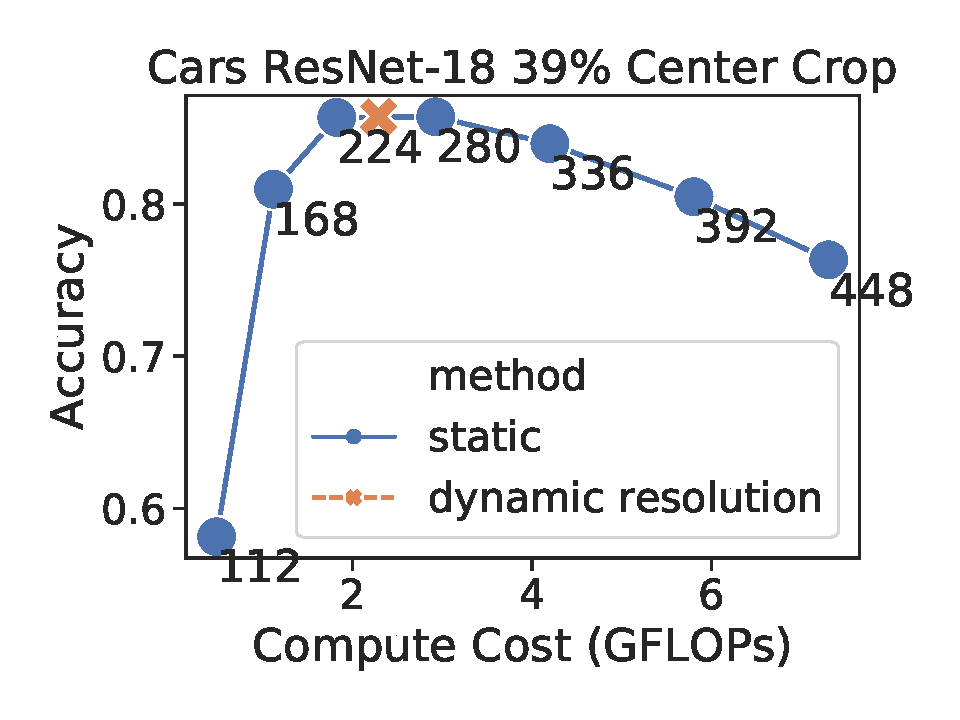
\includegraphics[width=0.195\textwidth]{asplos20-latex-template/figures/cars_resnet18_39_center.pdf} \\
    %\small (b)
    %\end{tabular}
    \begin{tabular}{@{}c@{}}
    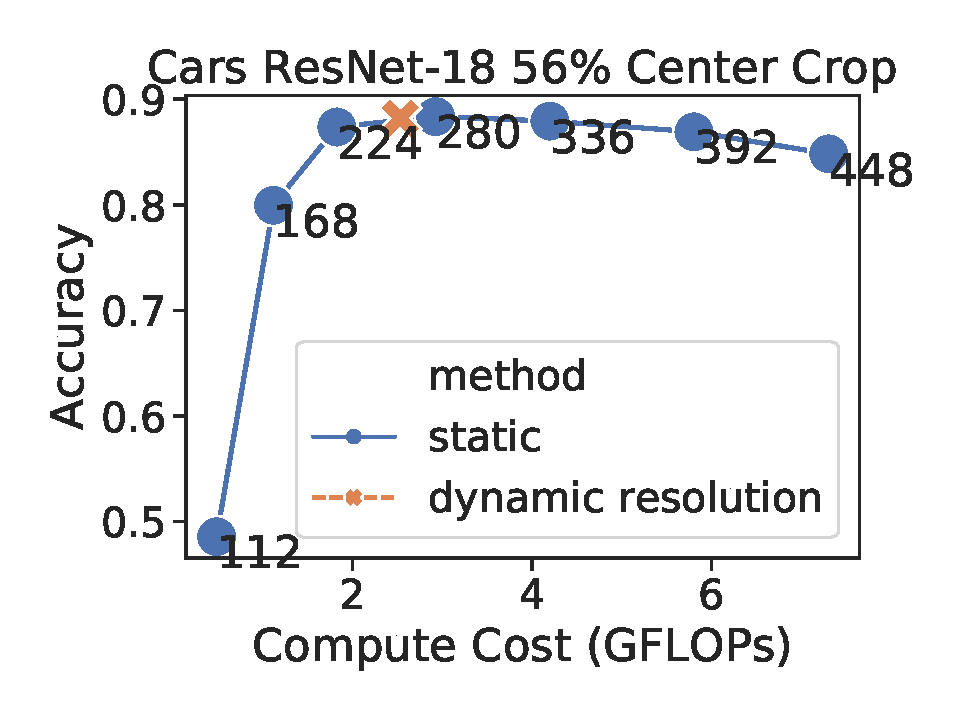
\includegraphics[width=0.45\textwidth]{e2e_figures/cars_resnet18_56_center.pdf} \\
    \small (b)
    \end{tabular}
    \begin{tabular}{@{}c@{}}
    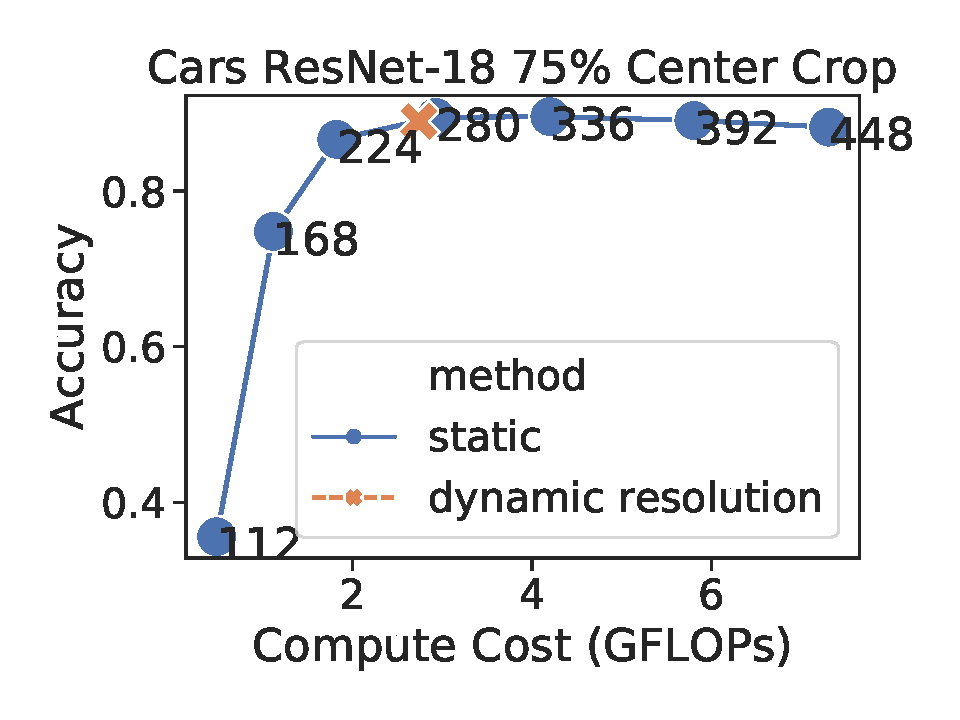
\includegraphics[width=0.45\textwidth]{e2e_figures/cars_resnet18_default_center.pdf} \\
    \small (c)
    \end{tabular}
    \begin{tabular}{@{}c@{}}
    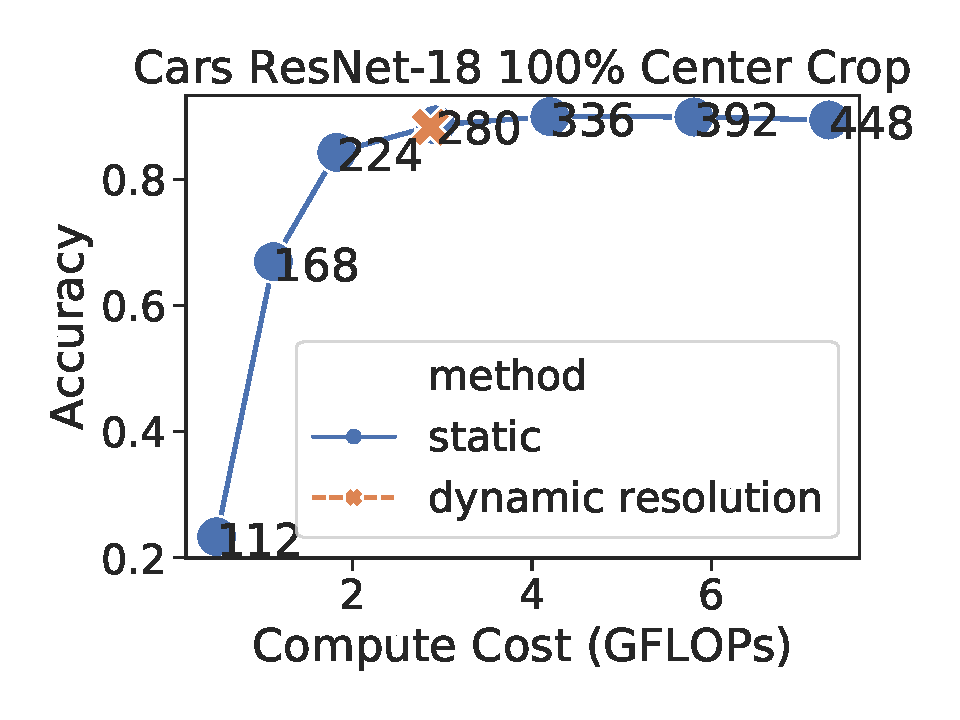
\includegraphics[width=0.45\textwidth]{e2e_figures/cars_resnet18_full_center.pdf} \\
    \small (d)
    \end{tabular}
    \begin{tabular}{@{}c@{}}
    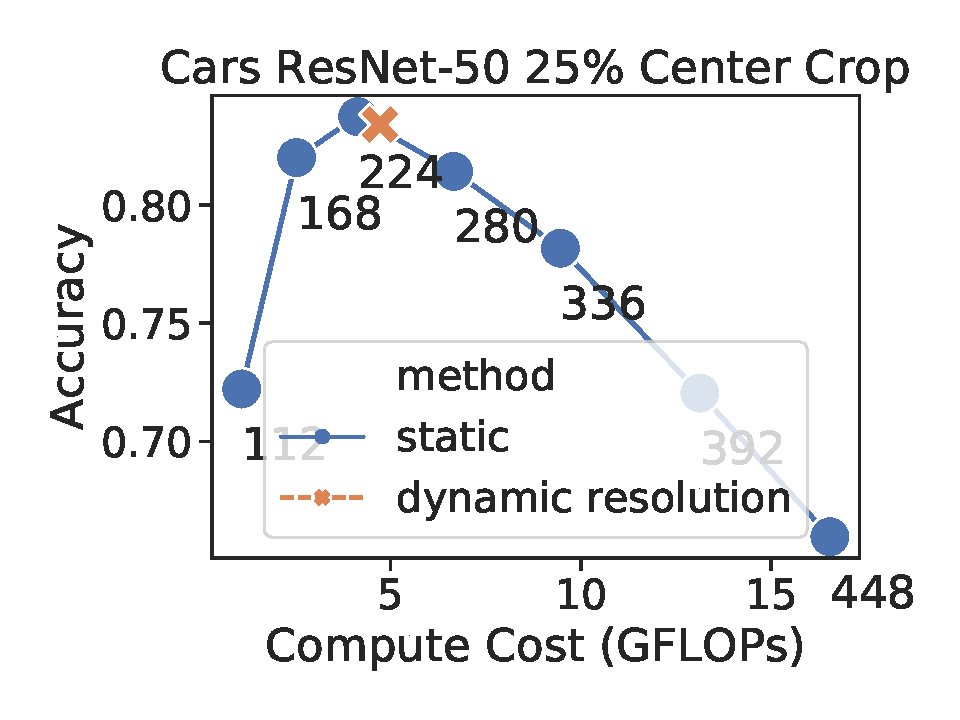
\includegraphics[width=0.45\textwidth]{e2e_figures/cars_resnet50_25_center.pdf} \\
    \small (e)
    \end{tabular}
    %\begin{tabular}{@{}c@{}}
    %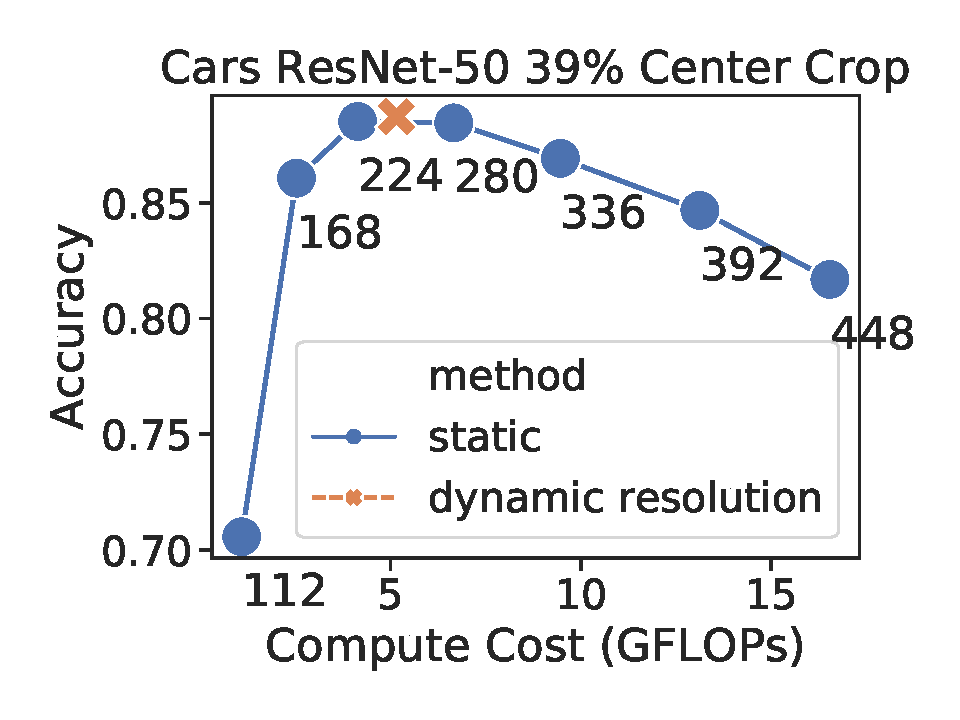
\includegraphics[width=0.195\textwidth]{asplos20-latex-template/figures/cars_resnet50_39_center.pdf} \\
    %\small (g)
    %\end{tabular}
    \begin{tabular}{@{}c@{}}
    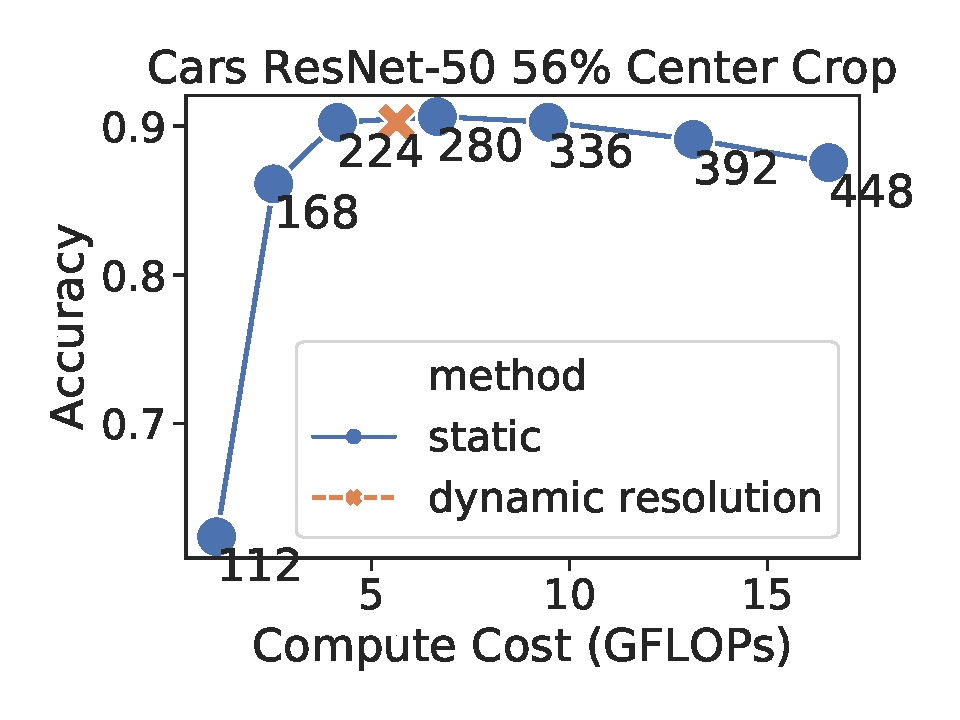
\includegraphics[width=0.45\textwidth]{e2e_figures/cars_resnet50_56_center.pdf} \\
    \small (f)
    \end{tabular}
    \begin{tabular}{@{}c@{}}
    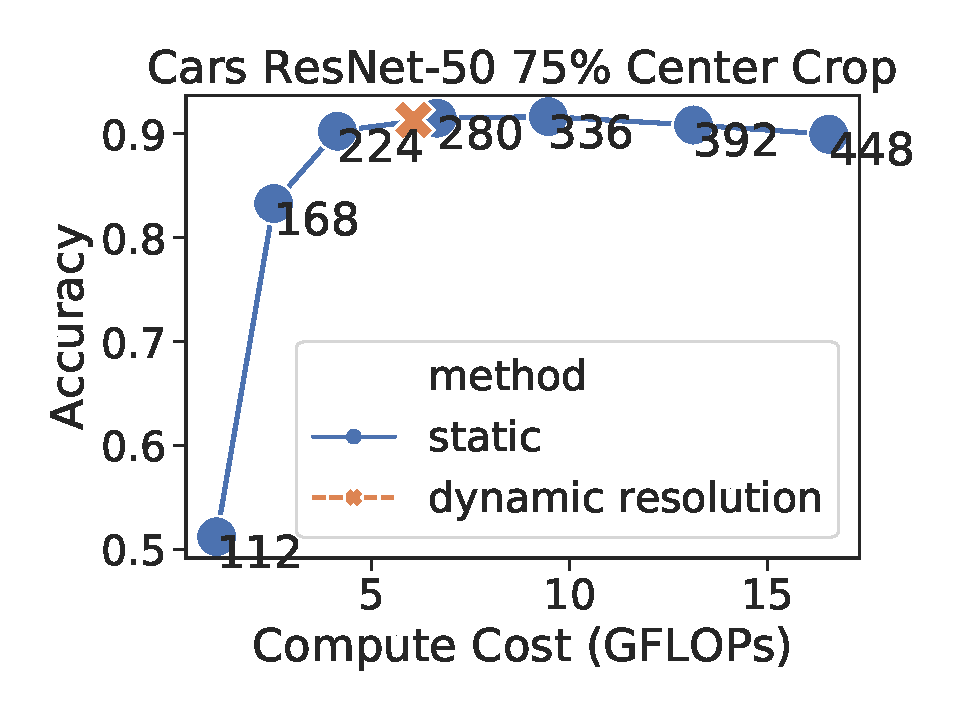
\includegraphics[width=0.45\textwidth]{e2e_figures/cars_resnet50_default_center.pdf} \\
    \small (g)
    \end{tabular}
    \begin{tabular}{@{}c@{}}
    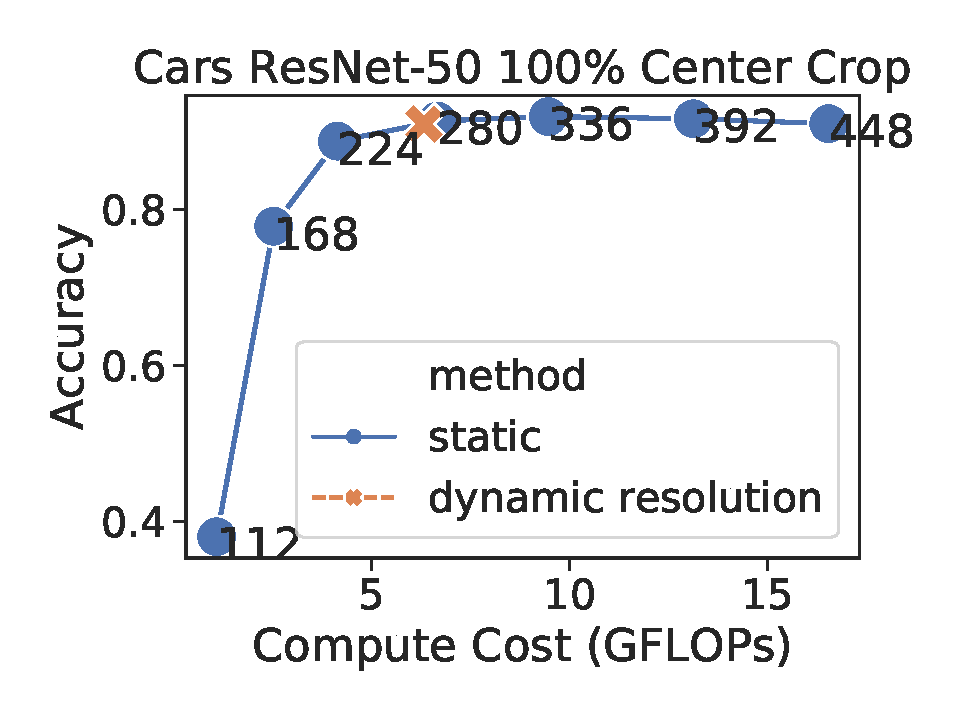
\includegraphics[width=0.45\textwidth]{e2e_figures/cars_resnet50_full_center.pdf} \\
    \small (h)
    \end{tabular}
    \caption{Accuracy vs. FLOPs comparison with static and dynamic resolution approaches using ResNet-18 (a-d) and 50 (e-h) on Stanford Cars. Crop sizes increase from left to right from 25\% on the left to 100\% on the right. Smaller crops favor lower resolutions more, while larger crops favor higher resolutions due to the models' dependence on object scale. The dynamic resolution approach operates at nearly the apex of every pareto curve, without hardcoding resolution.}
    \label{fig:accflops_resnet}
\end{figure*}
 To highlight the flexibility of a dynamic approach to resolution compared to static approaches that perform inference at a fixed resolution, we compare the accuracy of a dynamic resolution switching approach at several different center crop ratios (25\%, 39\%, 56\%, and ~75\%)\footnote{``75\%'' corresponds to the common practice of selecting a center crop (e.g., of 224 pixels from a $256\times256$ image, or 448 pixels from a $512\times512$ image), though the true area is closer to 77\%.}.
 Note that the best static choice of resolution changes for different crop sizes, as predicted by the ``train-test resolution discrepancy~\cite{touvron2019fixing}.''
While the choice of crop ratio is a evaluation hyperparameter, in practice it is unknown if a model is to be deployed on data from an unknown distribution of object sizes.
%Additionally, choosing the resolution corresponding to the best accuracy statically is optimistic because it assumes the distribution of object sizes at test time is known.

The dynamic resolution two model pipeline does not incur a significant overhead in compute complexity, as we use a lightweight, low-resolution architecture for the scale model (MobileNet v2)~\cite{sandler2018mobilenetv2}. 
We found in early experiments that predicting scale does not require fine-grained image details, and model accuracy did not vary significantly with the capacity of the model architecture (e.g., MobileNet vs. deep ResNets). 
In this case, the MobileNetv2 architecture used for the scale model corresponds to ~0.08 GFLOPs at $112\times112$ compared to the 1.8GFLOPs of ResNet-18 and 4.1GFLOPs of ResNet-50 at $224\times224$, an almost negligible amount of overhead.

\autoref{fig:accflops_resnet} shows the accuracy achieved by static and dynamic resolution approaches across a range of crop sizes on ImageNet.
On the ImageNet dataset, the best static resolution for the 56\%, 75\%, and 100\% center crops was $280\times280$, as expected due to the use of random cropping during training favors slightly larger object scales.
However, using the full crop (including \emph{more} of the image area) decreases model accuracy as object scales are biased towards smaller images.
The two-model dynamic resolution attains most of the accuracy of the best static resolution for each approach at a lower FLOP cost, and is pareto-optimal and near the apex of accuracy for most resolution configurations.
We note that the best static resolution at at 25\% crop drops, as expected, to $224\times224$, and the scale model adjusts accordingly. 

As expected, model accuracy is best for higher resolution inference when a larger crop size is used for evaluation and vice versa for lower resolution inference.
We point out the dramatic accuracy improvement achieved at the lowest resolution of ResNet-50 on Stanford Cars when switching from a default 75\% center crop to a 25\% crop; Top-1 accuracy improves from roughly 50\% to above 70\% for the smaller center crop.

Interestingly, while the general trends in the Accuracy vs. FLOPs curves for ImageNet and Stanford Cars are similar when comparing different crop sizes, there are several distinct differences in their shapes.
We note that the accuracy drop with small crops for higher resolutions is much more dramatic in Cars than on ImageNet.
At a 25\% center crop, the accuracy at $448\times448$ is \emph{lower} than at $112\times112$ for Cars, but it remains higher for ImageNet. 
Additionally, the accuracy gain at higher resolutions with larger center crops is much more modest in ImageNet (less than 1\%) than in Cars (up to 5\%).


\subsection{Accuracy vs. Storage Bandwidth}
\label{sec:storage}
We compare model accuracy and the amount of data read at several different crop sizes in \autoref{tab:imagenet_storage} and \autoref{tab:cars_storage}.
Here, the baseline approach reads the entirety of image data for every resolution.
Again, the best accuracy achieved by each approach depends on the crop size.
We find that the read savings on the validation set are highly data dependent, as was the case at calibration time (using training data).
Few inference resolutions on ImageNet reach above 20\% data savings, whereas many resolution/model configurations reach 40\% savings with minimal (< 0.1\%) accuracy loss.

Due to the quality threshold values being calibrated using the backbone model, the potential read bandwidth savings of the dynamic resolution approach are bounded by the amount of data used at $112\times112$ resolution (the resolution of the scale model).
It may be possible to reduce this limit by separately calibrating image quality for the scale model, as the scale model likely requires less image detail to discern object scales.

We observe the most accuracy losses when the amount of data read is limited at smaller crop sizes.
This trend can be attributed to our use of only 75\% center crops for calibration, and can likely be mitigated by calibrating quality thresholds for other crop scenarios, at the expense of additional compute cost.
Overall, however, we find that calibration generalizes well from the training set to the validation set, especially considering the simple image statistics computed by SSIM.
These results indicate that the savings depends on the classification task (the relevance of fine details for accuracy), as well as the distribution of resolution among the input resolutions.
We note that both the Cars and ImageNet dataset contain images only modestly higher resolution than $448\times448$ on average.

\begin{sidewaystable*}[t]
    \centering
    \begin{tabular}{c|}
    ImageNet\\
    Res \\
    \hline
    $112$ \\ 
    $168$ \\ 
    $224$ \\ 
    $280$ \\ 
    $336$ \\ 
    $392$ \\ 
    $448$ \\
    dynamic\\
    \end{tabular}
    \begin{tabular}{|c|c|}
    \multicolumn{2}{|c|}{ ResNet-18 75\% Crop}\\
    Default & Calibrated \\
    \hline
    47.8 & 47.7\\
    62.7 & 62.7\\ 
    69.5 & 69.5\\ 
    70.7 & 70.7\\ 
    70.1 & 70.1\\ 
    69.4 & 69.4\\ 
    68.9 & 69.0\\
    70.6 & 70.6\\ 
    \end{tabular}
    \begin{tabular}{|c|c|}
    \multicolumn{2}{|c|}{ ResNet-18 56\% Crop}\\
    Default & Calibrated  \\
    \hline
    49.9 & 49.8 \\ 
    62.9 & 62.8 \\ 
    68.7 & 68.7 \\ 
    69.6 & 69.5 \\ 
    68.6 & 68.5 \\ 
    67.4 & {\color{red}67.2} \\ 
    66.6 & 66.5 \\
    69.6 & {\color{red}69.4} \\ 
    \end{tabular}
    \begin{tabular}{|c|c|}
    \multicolumn{2}{|c|}{ ResNet-18 25\% Crop}\\
    Default & Calibrated  \\
    \hline
    49.4 & 49.3 \\ 
    57.7 & 57.7 \\ 
    61.4 & 61.4 \\ 
    60.9 & {\color{red} 60.7} \\ 
    58.2 & {\color{red} 57.5} \\ 
    55.3 & {\color{red} 54.7} \\ 
    52.9 & {\color{red} 52.6} \\
    61.5 & 61.5 \\ 
    \end{tabular}
    \begin{tabular}{|c}
    \\
    Read Savings \\
    \hline
    16.4\%\\ 
    5.1\%\\ 
    5.8\%\\ 
    20.2\%\\ 
    27.7\%\\ 
    17.8\%\\ 
    9.5\% \\
    11.2,10.6,8.6\%\\ 
    \end{tabular}

    \begin{tabular}{c|}
    ImageNet\\
    Res \\
    \hline
    $112$ \\ 
    $168$ \\ 
    $224$ \\ 
    $280$ \\ 
    $336$ \\ 
    $392$ \\ 
    $448$ \\
    dynamic\\
    \end{tabular}
    \begin{tabular}{|c|c|}
    \multicolumn{2}{|c|}{ ResNet-50 75\% Crop}\\
    Default & Calibrated \\
    \hline
    58.2 & 58.1\\
    70.5 & 70.5\\ 
    74.9 & 74.9\\ 
    76.0 & 76.0\\ 
    75.3 & 75.3\\ 
    74.7 & 74.7\\ 
    74.2 & 74.2\\
    75.7 & 75.6\\ 
    \end{tabular}
    \begin{tabular}{|c|c|}
    \multicolumn{2}{|c|}{ ResNet-50 56\% Crop}\\
    Default & Calibrated  \\
    \hline
    60.0 & 60.0\\ 
    70.5 & 70.5\\ 
    73.9 & 73.9\\ 
    74.5 & 74.6\\ 
    74.0 & 74.0\\ 
    73.2 & 73.1\\ 
    72.4 & 72.3\\
    74.3 & 74.3 \\ 
    \end{tabular}
    \begin{tabular}{|c|c|}
    \multicolumn{2}{|c|}{ ResNet-50 25\% Crop}\\
    Default & Calibrated  \\
    \hline
    58.5 & 58.5 \\ 
    65.4 & 65.4\\ 
    67.6 & 67.5\\ 
    67.1 & 67.0 \\ 
    65.8 & 65.7\\ 
    63.5 & 63.2 \\ 
    60.7 & {\color{red} 60.4}\\
    67.5 & 67.5 \\ 
    \end{tabular}
    \begin{tabular}{|c}
    \\
    Read Savings \\
    \hline
    7.4\%\\ 
    2.1\%\\ 
    8.9\%\\ 
    19.2\%\\ 
    6.2\%\\ 
    9.1\%\\ 
    8.0\% \\
    6.8,6.7,6.5\%\\ 
    \end{tabular}
    \caption{ImageNet read bandwidth savings; comparing accuracy when reading all data vs. reading the quantity of data according to storage calibration. Accuracy degradation > 0.1\% highlighted. Read savings for the dynamic pipeline are for each crop size.
    %Note that the read savings are identical for each crop size as we do not store pre-cropped versions of each image, opting instead to read a different number of scans for each image based on calibrated quality thresholds for each resolution.
    }
    \label{tab:imagenet_storage}
\end{sidewaystable*}


\begin{sidewaystable*}[t]
    \centering
    \begin{tabular}{c|}
    Cars \\
    Res \\
    \hline
    $112$ \\ 
    $168$ \\ 
    $224$ \\ 
    $280$ \\ 
    $336$ \\ 
    $392$ \\ 
    $448$ \\
    dynamic\\
    \end{tabular}
    \begin{tabular}{|c|c|}
    \multicolumn{2}{|c|}{ ResNet-18 75\% Crop}\\
    Default & Calibrated \\
    \hline
    35.6 & 35.6 \\
    74.8 & 74.7\\ 
    86.6 & 86.6\\ 
    89.4 & 89.4\\ 
    89.5 & 89.5\\ 
    89.0 & 89.0\\ 
    88.2 & 88.1\\
    88.9 & 88.9\\ 
    \end{tabular}
    \begin{tabular}{|c|c|}
    \multicolumn{2}{|c|}{ ResNet-18 56\% Crop}\\
    Default & Calibrated  \\
    \hline
    48.6 & 48.6 \\ 
    80.0 & {\color{red}79.6}\\ 
    87.4 & 87.3 \\ 
    88.4 & 88.4 \\ 
    87.9 & 88.0 \\ 
    86.9 & 86.9 \\ 
    84.8 & 84.7\\
    88.2& 88.2 \\ 
    \end{tabular}
    \begin{tabular}{|c|c|}
    \multicolumn{2}{|c|}{ ResNet-18 25\% Crop}\\
    Default & Calibrated  \\
    \hline
    63.2 & 63.1 \\ 
    77.6 & {\color{red}77.3}\\ 
    80.1 & 80.1\\ 
    77.9 & 77.9 \\ 
    71.3 & 71.4 \\ 
    63.8 & 63.8 \\ 
    56.0 & {\color{red}55.8} \\
    80.0 & 80.0 \\ 
    \end{tabular}
    \begin{tabular}{|c}
    \\
    Read Savings \\
    \hline
    31.8\%\\ 
    59.4\%\\ 
    20.5\%\\ 
    29.8\%\\ 
    31.4\%\\ 
    37.2\%\\ 
    43.0\% \\
    25.2,24.0,21.6\%\\ 
    \end{tabular}
    
    \begin{tabular}{c|}
    Cars\\
    Res \\
    \hline
    $112$ \\ 
    $168$ \\ 
    $224$ \\ 
    $280$ \\ 
    $336$ \\ 
    $392$ \\ 
    $448$ \\
    dynamic\\
    \end{tabular}
    \begin{tabular}{|c|c|}
    \multicolumn{2}{|c|}{ ResNet-50 75\% Crop}\\
    Default & Calibrated \\
    \hline
    51.2 & {\color{red} 50.8} \\
    83.3 & 83.3\\ 
    90.2 & 90.2\\ 
    91.5 & 91.4\\ 
    91.6 & 91.6\\ 
    90.8 & 90.8\\ 
    90.0 & 89.9\\
    91.3 & 91.2\\ 
    \end{tabular}
    \begin{tabular}{|c|c|}
    \multicolumn{2}{|c|}{ ResNet-50 56\% Crop}\\
    Default & Calibrated  \\
    \hline
    62.4 & {\color{red}62.0} \\ 
    86.1 & 86.1 \\ 
    90.3 & 90.2 \\ 
    90.6 & 90.6 \\ 
    90.3 & 90.3 \\ 
    89.1 & 89.1 \\ 
    87.6 & 87.5 \\
    90.3 & 90.2 \\ 
    \end{tabular}
    \begin{tabular}{|c|c|}
    \multicolumn{2}{|c|}{ ResNet-50 25\% Crop}\\
    Default & Calibrated  \\
    \hline
    72.2 & {\color{red} 71.5} \\ 
    82.0 & 81.9 \\ 
    83.7 & 83.6 \\ 
    81.4 & 81.4 \\ 
    78.2 & 78.1 \\ 
    72.0 & 71.9 \\ 
    66.0 & {\color{red}65.6} \\
    83.4 & 83.3 \\ 
    \end{tabular}
    \begin{tabular}{|c}
    \\
    Read Savings \\
    \hline
    68.8\%\\ 
    30.7\%\\ 
    40.9\%\\ 
    51.9\%\\ 
    6.5\%\\ 
    39.8\%\\ 
    49.3\% \\
    48.8,47.1,43.1\%\\ 
    \end{tabular}
    \caption{Cars read bandwidth savings; comparing accuracy when reading all data vs. reading the quantity of data according to storage calibration. Accuracy degradation > 0.1\% highlighted.
    Read savings for the dynamic pipeline are for each crop size.
    %Note that the read savings are identical for each crop size as we do not store pre-cropped versions of each image, opting instead to read a different number of scans for each image based on calibrated quality thresholds for each resolution.
    }
    \label{tab:cars_storage}
\end{sidewaystable*}
%\begin{figure}
%    \centering
%    \includegraphics{placeholderstorageMobileNetResnet50.png}
%    \caption{Caption}
%    \label{fig:my_label}
%\end{figure}
%\begin{figure}
%    \centering
%    \includegraphics{placeholderstorageMobileNetResnet18.png}
%    \caption{Caption}
%    \label{fig:my_label}
%\end{figure}

\section{Discussion}
In scenarios where the distribution of object scales at test time is well known, using a static model and the appropriate center crop size is likely to yield a good trade between accuracy and computational cost.
We see the dynamic resolution approach as being potentially most useful when some kind of load balancing or latency adjustment is desirable.
In such a scenario, one can adjust the crop size for evaluation to reduce the average computational cost of the model pipeline, as the scale model will automatically compensate for the change in object scale.
The scale model also has the advantage of improving the robustness of the pipeline to the distribution of object scales.
%TODO:  differences between ImageNet and Cars in storage calibration, possible explanations
However, the relationship between model accuracy, crop size, and input resolution is data and task-dependent.
%Increasing input resolution yields diminishing returns in accuracy, where we see gains fading more quickly in Cars than ImageNet.
At low resolutions, the effect of mismatched object scales (not balancing crop size with resolution) is much more pronounced in Cars.

From the perspective of read bandwidth from storage, we find substantial potential read bandwidth savings for both the Cars and ImageNet datasets.
Achieving the best savings/accuracy loss ratio will require tailoring storage calibration for each model/dataset scenario, but in our experience a small number of images ($\approx$30,000) is sufficient for calibration.
%Dataset and tasks-specific differences may be amplified when datasets comprise user-supplied images at much higher resolutions than are typical for curated ML datasets, or when classification tasks rely on different relevant features.

\paragraph{Quality Metrics}
We note that the use of structural similarity is a crude choice for image quality, especially for neural networks that favor quality metrics more in line with human perception~\cite{zhang2018unreasonable}.
Perhaps due to the choice of quality metric, a complicating issue occurs when higher resolutions potentially require \emph{lower} image quality or less image data than lower resolutions, further complicating the tradeoffs that can be made between accuracy, compute costs, and storage costs.
%In this work, we have chosen aggressive targets for accuracy, aiming for reducing image data reads only when less than 0.05\% accuracy is lost.
More sophisticated quality metrics that map better to neural network perceptual quality, as well as ones that are reference free~\cite{wang2011reduced} can potentially further improve bandwidth savings.
We have also made the implicit assumption that no image data is discarded from storage.
However, if an inference system is chosen such that the storage-accuracy and flops-accuracy tradeoff is to be made ahead of time, further savings can be obtained by (1) cropping images ahead of time, and (2) resizing them ahead of time losslessly.
Due to these factors, we consider the bandwidth savings a lower-bound on potential savings in the absence of further more domain information.

\paragraph{Alternative Loss Functions for the Scale Model}
%TODO: Observations of Storage calibration process, e.g., higher resolutions potentially requiring lower SSIM
We note that the current dynamic resolution model chooses resolutions solely based on their predicted accuracy given an input image.
It is possible to also incorporate inference costs (e.g., latency) for each resolution for further finetuning.
Still, using a two-model approach remains pareto-optimal in terms of accuracy vs. FLOPs while improving model accuracy over the default static resolution in most scenarios.



%TODO: Choosing an operating point on the pareto curve, potentially incorporating cost into the loss function.


%TODO: Lessons learned: like all thing machine learning, the best answer is likely data dependent or distribution dependent

\section{Related Work}
Improving the the computational efficiency of neural network inference (both with and without retraining) is a rapidly evolving field of research due to the high computational costs associated with modern convolutional architectures.
Frequently, these approaches introduce a quality--computational cost or accuracy--computational tradeoff space.
Beyond resolution, architecture agnostic approaches include exploiting quantization~\cite{rastegari2016xnor, zhou2016dorefa, fromm2020riptide}, weight pruning~\cite{ji2018tetris, frankle2018lottery}, input masking~\cite{yang2018energy}, temporal redundancy~\cite{buckler2018eva2}, model cascades~\cite{shen2017fast}, and alternative numerical representations~\cite{kim2016dynamic, lee2017energy, kalamkar2019study}.

The issue of scale dependence is an area of active research with model architecture~\cite{DBLP:journals/corr/KanazawaSJ14}, finetuning~\cite{touvron2019fixing}, data augmentation~\cite{hoffer2019mix}, and equivariance-based approaches~\cite{sosnovik2019scaleequivariant} being used.
While we present one of many possible motivations for multi-resolution models and one possible strategy for addressing the problem of scale dependence in vision models, the ability for an inference stack to flexibly switch between different image resolutions is useful.
Even in the ideal case of fully scale-equivariant models, image resolution remains a tunable hyperparameter dictating the amount of information or fine-grained detail in image in addition to the capacity of feature maps.
The overall approach of mapping image data to different resolutions and tuning resolution specific kernels is orthogonal to the motivation behind multi-resolution support.


An important requirement of efficient multi-resolution support is the availability of high performance kernel implementations for each combination of resolution, model, and hardware.
As the number of such possible combinations grows very quickly, we rely on work in automatic deep learning kernel optimizations ~\cite{ragan2013halide, chen2018tvm, zheng2020ansor, cowan2020automatic} to generate these kernels with minimal programmer effort.

Specializing storage with domain-specific knowledge for either increased capacity and performance is also an active area research~\cite{sampson2014approximate, jevdjic2017approximate, mazumdar2019vignette}.
Prior work has touched on cases where the relative importance of image data (e.g., critical format bits vs. noisy coefficient values) can be matched to storage at different levels of reliability~\cite{guo2016high, jevdjic2017approximate}.

Finally, our dynamic two-model pipeline draws inspiration from Mixture-of-Experts (MoE) approaches in machine learning~\cite{jacobs1991adaptive, shazeer2017outrageously, yang2019soft, lepikhin2020gshard}, where model architectures use a weighted combination of ``experts'' to increase model capacity.
Here, our two-model pipeline can be considered a modified MoE that uses weight-sharing, with the different experts being the different resolution variations of the backbone model.
While prior work has enforced sparse-weighting~\cite{shazeer2017outrageously} or soft-conditioning~\cite{yang2019soft} to efficiently implement the MoE, we use explicit control flow and train the scale and backbone models on separate objectives.

\section{Conclusion}
Image resolution is a fundamental hyperparameter in computer vision with ties to compute complexity, operator optimizations, and storage bandwidth.
The best choice of resolution also depends on other choices such as crop sizes and their effect on the distribution of object scales.
We systematically characterized the dependencies and relationships between these tradeoffs, and describe methods for maximizing efficiency with respect to compute and storage cost, encompassing both cases where resolution is a static choice and dynamic at inference time.

%\clearpage
%\bibliographystyle{plain}
%\bibliography{paper}
%
%
%\end{document}



